%%%%%%%%%%%%%%%%%%%%%%%%%%%%%%%%%%%%%%%%%%%%%%%%%%%
% Main Paper labels
\begin{filecontents*}{labels.aux} 
\relax 
\providecommand\hyper@newdestlabel[2]{}
\providecommand\zref@newlabel[2]{}
\providecommand\HyperFirstAtBeginDocument{\AtBeginDocument}
\HyperFirstAtBeginDocument{\ifx\hyper@anchor\@undefined
	\global\let\oldcontentsline\contentsline
	\gdef\contentsline#1#2#3#4{\oldcontentsline{#1}{#2}{#3}}
	\global\let\oldnewlabel\newlabel
	\gdef\newlabel#1#2{\newlabelxx{#1}#2}
	\gdef\newlabelxx#1#2#3#4#5#6{\oldnewlabel{#1}{{#2}{#3}}}
	\AtEndDocument{\ifx\hyper@anchor\@undefined
		\let\contentsline\oldcontentsline
		\let\newlabel\oldnewlabel
		\fi}
	\fi}
\global\let\hyper@last\relax 
\gdef\HyperFirstAtBeginDocument#1{#1}
\providecommand\HyField@AuxAddToFields[1]{}
\providecommand\HyField@AuxAddToCoFields[2]{}
\citation{abadie2010synthetic}
\citation{ferman2016revisiting}
\citation{ferman2018synthetic}
\citation{ferman2018cherry}
\citation{kaul2015synthetic}
\citation{klossner2017comparative}
\@writefile{toc}{\contentsline {section}{\numberline {1}Introduction}{1}{section.1}}
\citation{el1995}
\citation{cinar2017position}
\citation{dube2015pooling,xu2017generalized}
\citation{athey2017matrix}
\citation{doudchenko2016balancing,carvalho2018arco}
\citation{amjad2018robust}
\citation{neyman1923}
\@writefile{toc}{\contentsline {section}{\numberline {2}Counterfactual prediction}{3}{section.2}}
\newlabel{prediction}{{2}{3}{Counterfactual prediction}{section.2}{}}
\citation{imbens2015causal}
\citation{rubin1990}
\citation{athey2017matrix}
\citation{candes2009exact,candes2010matrix}
\citation{mazumder2010spectral}
\citation{athey2017matrix}
\@writefile{toc}{\contentsline {subsection}{\numberline {2.1}Relationship to matrix completion and covariate shift}{4}{subsection.2.1}}
\citation{yoon2018estimating}
\citation{athey2017matrix}
\citation{cortes2008sample}
\citation{huang2007correcting,ben2007analysis,bickel2009discriminative,cortes2010learning,2015arXiv150507818G}
\citation{schnabel2016recommendations}
\citation{johansson2016learning}
\citation{graves2012,goodfellow2016deep}
\@writefile{toc}{\contentsline {subsection}{\numberline {2.2}Nonparametric regression}{6}{subsection.2.2}}
\newlabel{eq:np}{{1}{6}{Nonparametric regression}{equation.2.1}{}}
\newlabel{eq:mse}{{2}{6}{Nonparametric regression}{equation.2.2}{}}
\newlabel{eq:pointwise}{{3}{6}{Nonparametric regression}{equation.2.3}{}}
\@writefile{toc}{\contentsline {section}{\numberline {3}RNNs for counteractual prediction}{6}{section.3}}
\newlabel{RNNs-section}{{3}{6}{RNNs for counteractual prediction}{section.3}{}}
\citation{lamb2016professor}
\citation{cho2014learning,bahdanau2014neural,vinyals2014grammar}
\citation{chorowski2015attention}
\citation{zhu2017deep}
\newlabel{eq:hidden}{{5}{7}{RNNs for counteractual prediction}{equation.3.5}{}}
\newlabel{rnn-obj}{{6}{7}{RNNs for counteractual prediction}{equation.3.6}{}}
\@writefile{toc}{\contentsline {subsection}{\numberline {3.1}Encoder-decoder networks}{7}{subsection.3.1}}
\citation{kingma2013auto}
\citation{fabius2014variational,chung2015recurrent,bowman2015generating}
\newlabel{eq:decoder}{{7}{8}{Encoder-decoder networks}{equation.3.7}{}}
\@writefile{toc}{\contentsline {subsection}{\numberline {3.2}Recurrent variational autoencoder}{8}{subsection.3.2}}
\citation{athey2017matrix}
\citation{abadie2010synthetic}
\citation{zou2005regularization,athey2017matrix}
\@writefile{toc}{\contentsline {section}{\numberline {4}Placebo tests}{9}{section.4}}
\newlabel{placebo}{{4}{9}{Placebo tests}{section.4}{}}
\citation{abadie2003economic}
\citation{abadie2003economic}
\citation{abadie2010synthetic}
\citation{abadie2010synthetic}
\citation{abadie2015comparative}
\citation{abadie2015comparative}
\citation{athey2017matrix}
\@writefile{toc}{\contentsline {subsection}{\numberline {4.1}Synthetic control datasets}{10}{subsection.4.1}}
\newlabel{synth-placebo}{{4.1}{10}{Synthetic control datasets}{subsection.4.1}{}}
\@writefile{lof}{\contentsline {figure}{\numberline {1}{\ignorespaces Placebo tests on California smoking data: {\tikz \draw [color={rgb:red,4;green,0;yellow,1}] (0,0) -- plot[mark=o, mark options={scale=2}] (0.25,0) -- (0.5,0);}, DID; {\tikz \draw [color={rgb:red,244;green,226;blue,66}] (0,0) -- plot[mark=triangle*, mark options={scale=2,fill=white}] (0.25,0) -- (0.5,0);}, ED; {\tikz \draw [color={rgb:red,0;green,5;blue,1}] (0,0) -- plot[mark=+, mark options={scale=2}] (0.25,0) -- (0.5,0);}, MC-NNM; {\tikz \draw [color={rgb:red,66;green,200;blue,244}] (0,0) -- plot[mark=x, mark options={scale=2}] (0.25,0) -- (0.5,0);}, RVAE; {\tikz \draw [color={rgb:red,66;green,107;blue,244}] (0,0) -- plot[mark=diamond, mark options={scale=2}] (0.25,0) -- (0.5,0);}, SCM; {\tikz \draw [color={rgb:red,244;pink,66;blue,223}] (0,0) -- plot[mark=triangle, mark options={scale=2, rotate=180}] (0.25,0) -- (0.5,0);}, VT-EN.\relax }}{11}{figure.caption.1}}
\newlabel{california-sim}{{1}{11}{Placebo tests on California smoking data: {\protect \tikz \protect \draw [color={rgb:red,4;green,0;yellow,1}] (0,0) -- plot[mark=o, mark options={scale=2}] (0.25,0) -- (0.5,0);}, DID; {\protect \tikz \protect \draw [color={rgb:red,244;green,226;blue,66}] (0,0) -- plot[mark=triangle*, mark options={scale=2,fill=white}] (0.25,0) -- (0.5,0);}, ED; {\protect \tikz \protect \draw [color={rgb:red,0;green,5;blue,1}] (0,0) -- plot[mark=+, mark options={scale=2}] (0.25,0) -- (0.5,0);}, MC-NNM; {\protect \tikz \protect \draw [color={rgb:red,66;green,200;blue,244}] (0,0) -- plot[mark=x, mark options={scale=2}] (0.25,0) -- (0.5,0);}, RVAE; {\protect \tikz \protect \draw [color={rgb:red,66;green,107;blue,244}] (0,0) -- plot[mark=diamond, mark options={scale=2}] (0.25,0) -- (0.5,0);}, SCM; {\protect \tikz \protect \draw [color={rgb:red,244;pink,66;blue,223}] (0,0) -- plot[mark=triangle, mark options={scale=2, rotate=180}] (0.25,0) -- (0.5,0);}, VT-EN.\relax }{figure.caption.1}{}}
\@writefile{toc}{\contentsline {subsection}{\numberline {4.2}Stock market data}{12}{subsection.4.2}}
\@writefile{lof}{\contentsline {figure}{\numberline {2}{\ignorespaces Placebo tests on stock market data: {\tikz \draw [color={rgb:red,4;green,0;yellow,1}] (0,0) -- plot[mark=o, mark options={scale=2}] (0.25,0) -- (0.5,0);}, DID; {\tikz \draw [color={rgb:red,244;green,226;blue,66}] (0,0) -- plot[mark=triangle*, mark options={scale=2,fill=white}] (0.25,0) -- (0.5,0);}, ED; {\tikz \draw [color={rgb:red,0;green,5;blue,1}] (0,0) -- plot[mark=+, mark options={scale=2}] (0.25,0) -- (0.5,0);}, MC-NNM; {\tikz \draw [color={rgb:red,66;green,200;blue,244}] (0,0) -- plot[mark=x, mark options={scale=2}] (0.25,0) -- (0.5,0);}, RVAE; {\tikz \draw [color={rgb:red,66;green,107;blue,244}] (0,0) -- plot[mark=diamond, mark options={scale=2}] (0.25,0) -- (0.5,0);}, SCM; {\tikz \draw [color={rgb:red,244;pink,66;blue,223}] (0,0) -- plot[mark=triangle, mark options={scale=2, rotate=180}] (0.25,0) -- (0.5,0);}, VT-EN.\relax }}{13}{figure.caption.2}}
\newlabel{stock-sim}{{2}{13}{Placebo tests on stock market data: {\protect \tikz \protect \draw [color={rgb:red,4;green,0;yellow,1}] (0,0) -- plot[mark=o, mark options={scale=2}] (0.25,0) -- (0.5,0);}, DID; {\protect \tikz \protect \draw [color={rgb:red,244;green,226;blue,66}] (0,0) -- plot[mark=triangle*, mark options={scale=2,fill=white}] (0.25,0) -- (0.5,0);}, ED; {\protect \tikz \protect \draw [color={rgb:red,0;green,5;blue,1}] (0,0) -- plot[mark=+, mark options={scale=2}] (0.25,0) -- (0.5,0);}, MC-NNM; {\protect \tikz \protect \draw [color={rgb:red,66;green,200;blue,244}] (0,0) -- plot[mark=x, mark options={scale=2}] (0.25,0) -- (0.5,0);}, RVAE; {\protect \tikz \protect \draw [color={rgb:red,66;green,107;blue,244}] (0,0) -- plot[mark=diamond, mark options={scale=2}] (0.25,0) -- (0.5,0);}, SCM; {\protect \tikz \protect \draw [color={rgb:red,244;pink,66;blue,223}] (0,0) -- plot[mark=triangle, mark options={scale=2, rotate=180}] (0.25,0) -- (0.5,0);}, VT-EN.\relax }{figure.caption.2}{}}
\citation{meyer1979public,alesina2013nation,bandiera2018nation}
\citation{engerman2005evolution}
\citation{acemoglu2008persistence,besley2009origins}
\citation{galor2009inequality}
\@writefile{toc}{\contentsline {section}{\numberline {5}Application: Homestead policy and public schooling}{14}{section.5}}
\newlabel{schooling-app}{{5}{14}{Application: Homestead policy and public schooling}{section.5}{}}
\citation{sylla1993sources}
\citation{sylla1995sourcesa,sylla1995sourcesb}
\citation{haines2010}
\citation{williamson2017seven}
\citation{haines2010}
\citation{haines2010}
\citation{atack2013use}
\@writefile{toc}{\contentsline {subsection}{\numberline {5.1}Data and assumptions}{15}{subsection.5.1}}
\newlabel{educ-data}{{5.1}{15}{Data and assumptions}{subsection.5.1}{}}
\@writefile{toc}{\contentsline {subsection}{\numberline {5.2}Estimates}{16}{subsection.5.2}}
\citation{gates1941land,gates1979federal}
\citation{snyder2010digest}
\@writefile{lof}{\contentsline {figure}{\numberline {3}{\ignorespaces Encoder-decoder estimates of the impact of the HSA on state government education spending, 1809 to 1982: {\color  {Darjeeling15}{\sampleline  {}}}, observed treated; {\color  {Darjeeling11}{\sampleline  {dashed}}}, observed control; {\color  {Darjeeling15}{\sampleline  {dotted}}}, counterfactual treated; {\color  {Darjeeling15}{\sampleline  {dash pattern=on .7em off .2em on .05em off .2em}}}, $\boldsymbol  {\mathaccentV {bar}016{\upphi }^{(t)}}$.\relax }}{18}{figure.caption.3}}
\newlabel{educ-ed}{{3}{18}{Encoder-decoder estimates of the impact of the HSA on state government education spending, 1809 to 1982: {\color {Darjeeling15}{\sampleline {}}}, observed treated; {\color {Darjeeling11}{\sampleline {dashed}}}, observed control; {\color {Darjeeling15}{\sampleline {dotted}}}, counterfactual treated; {\color {Darjeeling15}{\sampleline {dash pattern=on .7em off .2em on .05em off .2em}}}, $\boldsymbol {\bar {\upphi }^{(t)}}$.\relax }{figure.caption.3}{}}
\citation{yoon2018estimating}
\@writefile{toc}{\contentsline {section}{\numberline {6}Conclusion}{19}{section.6}}
\newlabel{conclusion}{{6}{19}{Conclusion}{section.6}{}}
\bibstyle{rss}
\bibdata{rnns-causal}
\bibcite{abadie2010synthetic}{{1}{2010}{{Abadie et~al.}}{{Abadie, Diamond and Hainmueller}}}
\bibcite{abadie2015comparative}{{2}{2015}{{Abadie et~al.}}{{Abadie, Diamond and Hainmueller}}}
\bibcite{abadie2003economic}{{3}{2003}{{Abadie and Gardeazabal}}{{}}}
\bibcite{acemoglu2008persistence}{{4}{2008}{{Acemoglu and Robinson}}{{}}}
\bibcite{alesina2013nation}{{5}{2013}{{Alesina et~al.}}{{Alesina, Giuliano and Reich}}}
\bibcite{amjad2018robust}{{6}{2018}{{Amjad et~al.}}{{Amjad, Shah and Shen}}}
\bibcite{atack2013use}{{7}{2013}{{Atack}}{{}}}
\bibcite{athey2017matrix}{{8}{2017}{{{Athey} et~al.}}{{{Athey}, {Bayati}, {Doudchenko}, {Imbens} and {Khosravi}}}}
\bibcite{bahdanau2014neural}{{9}{2014}{{{Bahdanau} et~al.}}{{{Bahdanau}, {Cho} and {Bengio}}}}
\bibcite{bandiera2018nation}{{10}{2018}{{Bandiera et~al.}}{{Bandiera, Mohnen, Rasul and Viarengo}}}
\bibcite{ben2007analysis}{{11}{2007}{{Ben-David et~al.}}{{Ben-David, Blitzer, Crammer and Pereira}}}
\bibcite{besley2009origins}{{12}{2009}{{Besley and Persson}}{{}}}
\bibcite{bickel2009discriminative}{{13}{2009}{{Bickel et~al.}}{{Bickel, Br{\"u}ckner and Scheffer}}}
\bibcite{bowman2015generating}{{14}{2015}{{{Bowman} et~al.}}{{{Bowman}, {Vilnis}, {Vinyals}, {Dai}, {Jozefowicz} and {Bengio}}}}
\bibcite{candes2010matrix}{{15}{2010}{{Cand{\`e}s and Plan}}{{}}}
\bibcite{candes2009exact}{{16}{2009}{{Cand{\`e}s and Recht}}{{}}}
\bibcite{carvalho2018arco}{{17}{2018}{{Carvalho et~al.}}{{Carvalho, Masini and Medeiros}}}
\bibcite{cavallo2013catastrophic}{{18}{2013}{{Cavallo et~al.}}{{Cavallo, Galiani, Noy and Pantano}}}
\bibcite{cho2014learning}{{19}{2014}{{{Cho} et~al.}}{{{Cho}, {van Merrienboer}, {Gulcehre}, {Bahdanau}, {Bougares}, {Schwenk} and {Bengio}}}}
\bibcite{chollet2015keras}{{20}{2015}{{Chollet}}{{}}}
\bibcite{chorowski2015attention}{{21}{2015}{{Chorowski et~al.}}{{Chorowski, Bahdanau, Serdyuk, Cho and Bengio}}}
\bibcite{chung2014}{{22}{2014}{{{Chung} et~al.}}{{{Chung}, {Gulcehre}, {Cho} and {Bengio}}}}
\bibcite{chung2015recurrent}{{23}{2015}{{Chung et~al.}}{{Chung, Kastner, Dinh, Goel, Courville and Bengio}}}
\bibcite{cinar2017position}{{24}{2017}{{Cinar et~al.}}{{Cinar, Mirisaee, Goswami, Gaussier, A{\"i}t-Bachir and Strijov}}}
\bibcite{cortes2010learning}{{25}{2010}{{Cortes et~al.}}{{Cortes, Mansour and Mohri}}}
\bibcite{cortes2008sample}{{26}{2008}{{Cortes et~al.}}{{Cortes, Mohri, Riley and Rostamizadeh}}}
\bibcite{doudchenko2016balancing}{{27}{2016}{{{Doudchenko} and {Imbens}}}{{}}}
\bibcite{dube2015pooling}{{28}{2015}{{Dube and Zipperer}}{{}}}
\bibcite{el1995}{{29}{1995}{{El~Hihi and Bengio}}{{}}}
\bibcite{engerman2005evolution}{{30}{2005}{{Engerman and Sokoloff}}{{}}}
\bibcite{fabius2014variational}{{31}{2014}{{{Fabius} and {van Amersfoort}}}{{}}}
\bibcite{ferman2016revisiting}{{32}{2016}{{Ferman and Pinto}}{{}}}
\bibcite{ferman2018synthetic}{{33}{2018}{{Ferman and Pinto}}{{}}}
\bibcite{ferman2018cherry}{{34}{2018}{{Ferman et~al.}}{{Ferman, Pinto and Possebom}}}
\bibcite{firpo2018synthetic}{{35}{2018}{{Firpo and Possebom}}{{}}}
\bibcite{galor2009inequality}{{36}{2009}{{Galor et~al.}}{{Galor, Moav and Vollrath}}}
\bibcite{2015arXiv150507818G}{{37}{2015}{{{Ganin} et~al.}}{{{Ganin}, {Ustinova}, {Ajakan}, {Germain}, {Larochelle}, {Laviolette}, {Marchand} and {Lempitsky}}}}
\bibcite{gates1941land}{{38}{1941}{{Gates}}{{}}}
\bibcite{gates1979federal}{{39}{1979}{{Gates}}{{}}}
\bibcite{glorot2010}{{40}{2010}{{Glorot and Bengio}}{{}}}
\bibcite{goodfellow2016deep}{{41}{2016}{{Goodfellow et~al.}}{{Goodfellow, Bengio and Courville}}}
\bibcite{graves2012}{{42}{2012}{{Graves}}{{}}}
\bibcite{hahn2017synthetic}{{43}{2017}{{Hahn and Shi}}{{}}}
\bibcite{haines2010}{{44}{2010}{{Haines}}{{}}}
\bibcite{huang2007correcting}{{45}{2007}{{Huang et~al.}}{{Huang, Gretton, Borgwardt, Sch{\"o}lkopf and Smola}}}
\bibcite{imbens2015causal}{{46}{2015}{{Imbens and Rubin}}{{}}}
\bibcite{johansson2016learning}{{47}{2016}{{Johansson et~al.}}{{Johansson, Shalit and Sontag}}}
\bibcite{kaul2015synthetic}{{48}{2015}{{Kaul et~al.}}{{Kaul, Kl{\"o}{\ss }ner, Pfeifer and Schieler}}}
\bibcite{kingma2014adam}{{49}{2014}{{{Kingma} and {Ba}}}{{}}}
\bibcite{kingma2013auto}{{50}{2013}{{{Kingma} and {Welling}}}{{}}}
\bibcite{klossner2017comparative}{{51}{2017}{{Kl{\"o}{\ss }ner et~al.}}{{Kl{\"o}{\ss }ner, Kaul, Pfeifer and Schieler}}}
\bibcite{lamb2016professor}{{52}{2016}{{Lamb et~al.}}{{Lamb, Goyal, Zhang, Zhang, Courville and Bengio}}}
\bibcite{mazumder2010spectral}{{53}{2010}{{Mazumder et~al.}}{{Mazumder, Hastie and Tibshirani}}}
\bibcite{meyer1979public}{{54}{1979}{{Meyer et~al.}}{{Meyer, Tyack, Nagel and Gordon}}}
\bibcite{neyman1923}{{55}{1923}{{Neyman}}{{}}}
\citation{splawa1990}
\bibcite{rubin1990}{{56}{1990}{{Rubin}}{{}}}
\bibcite{schmidhuber1997long}{{57}{1997}{{Schmidhuber and Hochreiter}}{{}}}
\bibcite{schnabel2016recommendations}{{58}{2016}{{{Schnabel} et~al.}}{{{Schnabel}, {Swaminathan}, {Singh}, {Chandak} and {Joachims}}}}
\bibcite{snyder2010digest}{{59}{2010}{{Snyder and Dillow}}{{}}}
\bibcite{splawa1990}{{60}{1990}{{Splawa-Neyman et~al.}}{{Splawa-Neyman, Dabrowska, Speed et~al.}}}
\bibcite{sylla1993sources}{{61}{1993}{{Sylla et~al.}}{{Sylla, Legler and Wallis}}}
\bibcite{sylla1995sourcesa}{{62}{1995{a}}{{Sylla et~al.}}{{Sylla, Legler and Wallis}}}
\bibcite{sylla1995sourcesb}{{63}{1995{b}}{{Sylla et~al.}}{{Sylla, Legler and Wallis}}}
\bibcite{vinyals2014grammar}{{64}{2014}{{{Vinyals} et~al.}}{{{Vinyals}, {Kaiser}, {Koo}, {Petrov}, {Sutskever} and {Hinton}}}}
\bibcite{williamson2017seven}{{65}{2017}{{Williamson}}{{}}}
\bibcite{xu2017generalized}{{66}{2017}{{Xu}}{{}}}
\bibcite{yoon2018estimating}{{67}{2018}{{Yoon et~al.}}{{Yoon, Zame and van~der Schaar}}}
\bibcite{zhu2017deep}{{68}{2017}{{{Zhu} and {Laptev}}}{{}}}
\bibcite{zou2005regularization}{{69}{2005}{{Zou and Hastie}}{{}}}
\end{filecontents*}
%%%%%%%%%%%%%%%%%%%%%%%%%%%%%%%%%%%%%%%%%%%%%%%%%%%

\title{Web-Based Supporting Materials for\\
	``RNN-based counterfactual prediction'' by Jason Poulos}

\date{}

%%%%%%%%%%%%%%%%%%%%%%%%%%%%%%%%%%%%%%%%%%%%%%%%%%
% Set document class
\documentclass[hidelinks,12pt]{article}

% Define packages
\usepackage{hyperref, url} 
\usepackage{graphicx,amsfonts,psfrag,layout,subcaption,array,longtable,lscape,booktabs,dcolumn,amsmath,amssymb,amssymb,amsthm,setspace,epigraph,chronology,color,colortbl,caption,wasysym,diagbox,natbib,colortbl,upgreek}
\usepackage[]{graphicx}\usepackage[]{color}
\usepackage[page]{appendix}
\usepackage[section]{placeins}
\usepackage[linewidth=1pt]{mdframed}
\usepackage[margin={1in}]{geometry} %1 inch margins

%% Reference labels in the online appendix
\usepackage{xr}
\externaldocument{labels}

% Footnotes stick at the bottom
\usepackage[bottom]{footmisc}

% Caption keys
\usepackage{mathtools,tikz,caption}
\captionsetup{labelfont=sc,labelsep=period}
\DeclareRobustCommand\sampleline[1]{%
	\tikz\draw[#1] (0,0) (0,\the\dimexpr\fontdimen22\textfont2\relax)
	-- (2em,\the\dimexpr\fontdimen22\textfont2\relax);%
}

\usetikzlibrary{plotmarks}

% Wes Anderson colors

\usepackage{xcolor}

\definecolor{Darjeeling11}{HTML}{FF0000}
\definecolor{Darjeeling15}{HTML}{5BBCD6}

% New footnote characters
\usepackage{footmisc}
\DefineFNsymbols{mySymbols}{{\ensuremath\dagger}{\ensuremath\ddagger}\S\P
	*{**}{\ensuremath{\dagger\dagger}}{\ensuremath{\ddagger\ddagger}}}
\setfnsymbol{mySymbols}

% New tabular environment
\usepackage{tabularx}
\newcolumntype{Y}{>{\raggedleft\arraybackslash}X}% raggedleft column X

% Define appendix 
\renewcommand*\appendixpagename{Appendix}
\renewcommand*\appendixtocname{Appendix}

% Position floats
\renewcommand{\textfraction}{0.05}
\renewcommand{\topfraction}{0.95}
\renewcommand{\bottomfraction}{0.95}
\renewcommand{\floatpagefraction}{0.35}
\setcounter{totalnumber}{5}

% Colors for highlighting tables
\definecolor{Gray}{gray}{0.9}

% Different font in captions
\newcommand{\captionfonts}{\normalsize}

\makeatletter  % Allow the use of @ in command names
\long\def\@makecaption#1#2{%
	\vskip\abovecaptionskip
	\sbox\@tempboxa{{\captionfonts #1: #2}}%
	\ifdim \wd\@tempboxa >\hsize
	{\captionfonts #1: #2\par}
	\else
	\hbox to\hsize{\hfil\box\@tempboxa\hfil}%
	\fi
	\vskip\belowcaptionskip}
%\makeatother   % Cancel the effect of \makeatletter

% Set Spacing
%\doublespacing

% Number assumptions
\newtheorem*{assumption*}{\assumptionnumber}
\providecommand{\assumptionnumber}{}
\makeatletter
\newenvironment{assumption}[2]
{%
	\renewcommand{\assumptionnumber}{Assumption #1}%
	\begin{assumption*}%
		\protected@edef\@currentlabel{#1}%
	}
	{%
	\end{assumption*}
}
\makeatother

% Macros
\newcommand{\Adv}{{\mathbf{Adv}}}       
\newcommand{\prp}{{\mathrm{prp}}}                  % How to define new commands 
\newcommand{\calK}{{\cal K}}
\newcommand{\outputs}{{\Rightarrow}}                
\newcommand{\getsr}{{\:\stackrel{{\scriptscriptstyle\hspace{0.2em}\$}}{\leftarrow}\:}}
\newcommand{\andthen}{{\::\;\;}}    %  \: \; for thinspace, medspace, thickspace
\newcommand{\Rand}[1]{{\mathrm{Rand}[{#1}]}}       % A command with one argument
\newcommand{\Perm}[1]{{\mathrm{Perm}[{#1}]}}       
\newcommand{\Randd}[2]{{\mathrm{Rand}[{#1},{#2}]}} % and with two arguments
\newcommand{\E}{\mathrm{E}}
\newcommand{\Var}{\mathrm{Var}}
\newcommand{\Cov}{\mathrm{Cov}}
\DeclareMathOperator*{\plim}{plim}
\newcommand\independent{\protect\mathpalette{\protect\independenT}{\perp}}
\def\independenT#1#2{\mathrel{\rlap{$#1#2$}\mkern2mu{#1#2}}}
\newcommand{\possessivecite}[1]{\citeauthor{#1}'s [\citeyear{#1}]} 

\renewcommand*\contentsname{Table of contents}

%%%%%%%%%%%%%%%%%%%%%%%%%%%%%%%%%%%%%%%%%%%%%%%%%%%%%%%%%%%%%%%%%%%%%%%%%%%%

\begin{document}

\begin{singlespacing}
\maketitle \thispagestyle{empty}
\tableofcontents \thispagestyle{empty}
\end{singlespacing}

\pagenumbering{roman}% Roman-numbered pages (start from i)

\pagebreak
\pagenumbering{arabic}% Arabic-numbered pages (start from 1)

\section{Implementation details} \label{imp}

The networks are implemented with the \texttt{Keras} neural network library \citep{chollet2015keras} in Python on top of a TensorFlow backend. When implementing encoder-decoder networks, the encoder takes the form of a two-layer Long Short-Term Memory (LSTM) network \citep{schmidhuber1997long}, each with 128 hidden units, and the decoder is a single-layer Gated Recurrent Unit (GRU) \citep{chung2014} also with 128 hidden units. Each recurrent layer uses a linear activation function ($f_1$) with weights initialized using Xavier initialization \citep{glorot2010}. The loss function internally computes the predicted outputs as a linear function ($f_2$) of the log probabilities. 

RNN weights are learned with mini-batch gradient descent on the WMSE using \texttt{Adam} stochastic optimization with the learning rate set to $5\,\cdot\,10^{-4}$ \citep{kingma2014adam}. As a regularization strategy, I apply dropout to the inputs and L2 regularization losses to the network weights. The networks are trained for 1,000 epochs, which takes 10 minutes to run on a laptop CPU. The model is validated on the last 20\% of the training set input-out pairs.  

The RVAE is implemented similarly, but with the following differences: the encoder takes the form of a single-layer LSTM with 32 hidden units and the decoder is a two-layer LSTM with the number of hidden units equal to 32 and the number of predictors, respectively. The latent space $\boldsymbol{z}$ is implemented as a densely-connected layer with a dimension of 200 units and $f_3(\cdot)$ takes the form of a log-normal distribution. The RVAE is trained with stochastic gradient descent for 5,000 epochs, which takes seven minutes to run on the same CPU.

\clearpage
\section{Hypothesis testing} \label{eval}

\citet{abadie2010synthetic} propose a randomization inference approach for calculating the exact distribution of placebo effects under the sharp null hypothesis of no effect. \citet{cavallo2013catastrophic} extends the placebo-based testing approach to the case of multiple (placebo) treated units by constructing a distribution of \emph{average} placebo effects under the null hypothesis. \citet{firpo2018synthetic} derive the conditions under which the randomization inference approach is valid from a finite sample perspective and \citet{hahn2017synthetic} analyze the approach from a repeated sampling perspective.

Randomization $p$-values are obtained following these steps:

\begin{enumerate} 
	\item Estimate the observed test static $\boldsymbol{\hat{\upphi}}$ from (\ref{eq:pointwise}). Averaging over the time dimension results in a $\text{T}_\star$-length array of observed average treatment effects. 
	\item Calculate every possible average placebo treated effect $\upmu$ by randomly sampling without replacement which $\text{J}-1$ control units are assumed to be treated. There are $\mathcal{Q} = \sum\limits_{\text{g}=1}^{\text{J}-1} {\text{J} \choose \text{g}}$ possible average placebo effects. Since calculating $\mathcal{Q}$ can be computationally burdensome for relatively high values of $J$, I artificially set $\mathcal{Q} = 10,000$ in cases when $\text{J} > 16$. The result is a matrix of dimension $\mathcal{Q} \times \text{T}_\star$
	\item Sum over the time dimension the number of $\upmu$ that are greater than or equal to $\boldsymbol{\hat{\upphi}}$.  \label{counts}
\end{enumerate}

Each element of the vector obtained from Step \ref{counts} is divided by $\mathcal{Q}$ to estimate a $\text{T}_\star$-length vector of exact two-sided $p$ values, $\hat{p}$. 

\subsection{Randomization confidence intervals}

Under the assumption that treatment has a constant additive effect $\Delta$, I construct an interval estimate for $\Delta$ by inverting the randomization test. Let $\updelta_\Delta$ be the test statistic calculated by subtracting all possible $\upmu$ by $\Delta$. I derive a two-sided randomization confidence interval by collecting all values of $\updelta_\Delta$ that yield $\hat{p}$ values greater than or equal to significance level $\upalpha=0.05$. I find the endpoints of the confidence interval by randomly sampling 500 values of $\Delta$.

\clearpage
\section{Supporting Figures}

\begin{figure}[htbp]
	\centering
	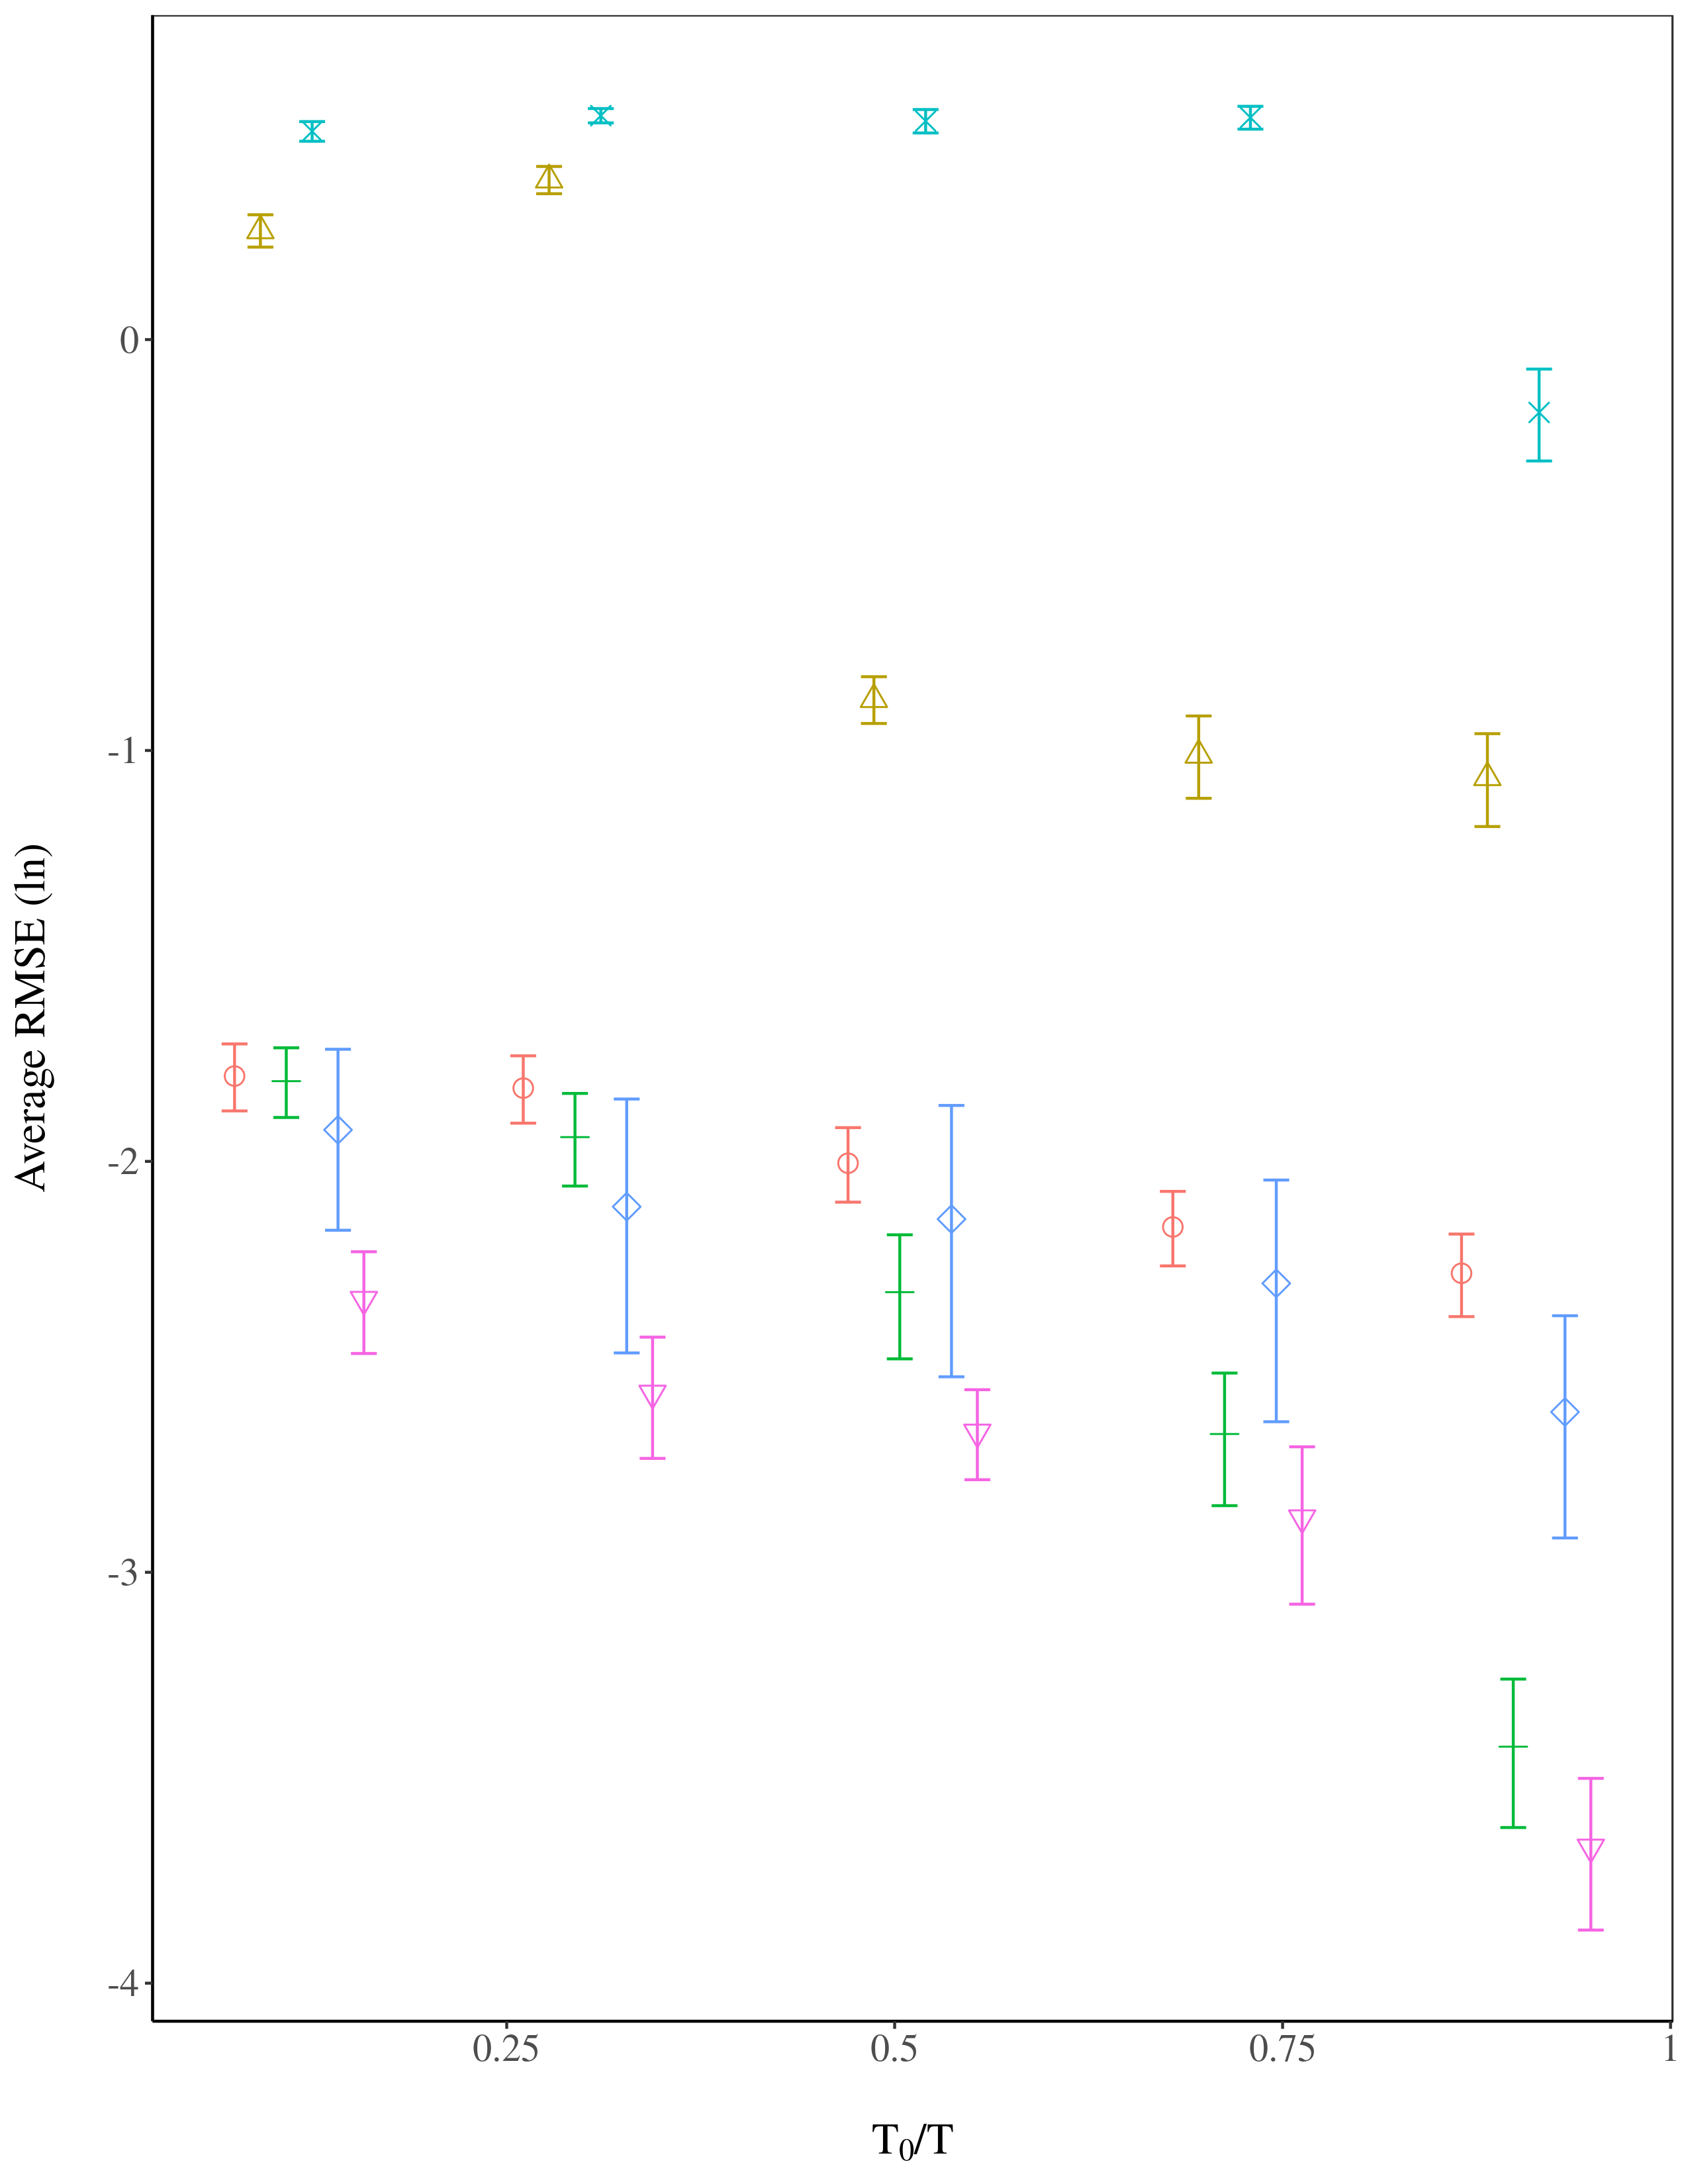
\includegraphics[width=0.9\textwidth]{plots/basque-sim.png}
	\caption{Placebo tests on Basque Country terrorism data: 
		{\protect\tikz \protect\draw[color={rgb:red,4;green,0;yellow,1}] (0,0) -- plot[mark=o, mark options={scale=2}] (0.25,0) -- (0.5,0);}, DID;
		{\protect\tikz \protect\draw[color={rgb:red,244;green,226;blue,66}] (0,0) -- plot[mark=triangle*, mark options={scale=2,fill=white}] (0.25,0) -- (0.5,0);}, ED; 
		{\protect\tikz \protect\draw[color={rgb:red,0;green,5;blue,1}] (0,0) -- plot[mark=+, mark options={scale=2}] (0.25,0) -- (0.5,0);}, MC-NNM;
		{\protect\tikz \protect\draw[color={rgb:red,66;green,200;blue,244}] (0,0) -- plot[mark=x, mark options={scale=2}] (0.25,0) -- (0.5,0);}, RVAE;
		{\protect\tikz \protect\draw[color={rgb:red,66;green,107;blue,244}] (0,0) -- plot[mark=diamond, mark options={scale=2}] (0.25,0) -- (0.5,0);}, SCM;
		{\protect\tikz \protect\draw[color={rgb:red,244;pink,66;blue,223}] (0,0) -- plot[mark=triangle, mark options={scale=2, rotate=180}] (0.25,0) -- (0.5,0);}, VT-EN.\label{basque-sim}}
\end{figure}

\begin{figure}[htbp]
	\centering
	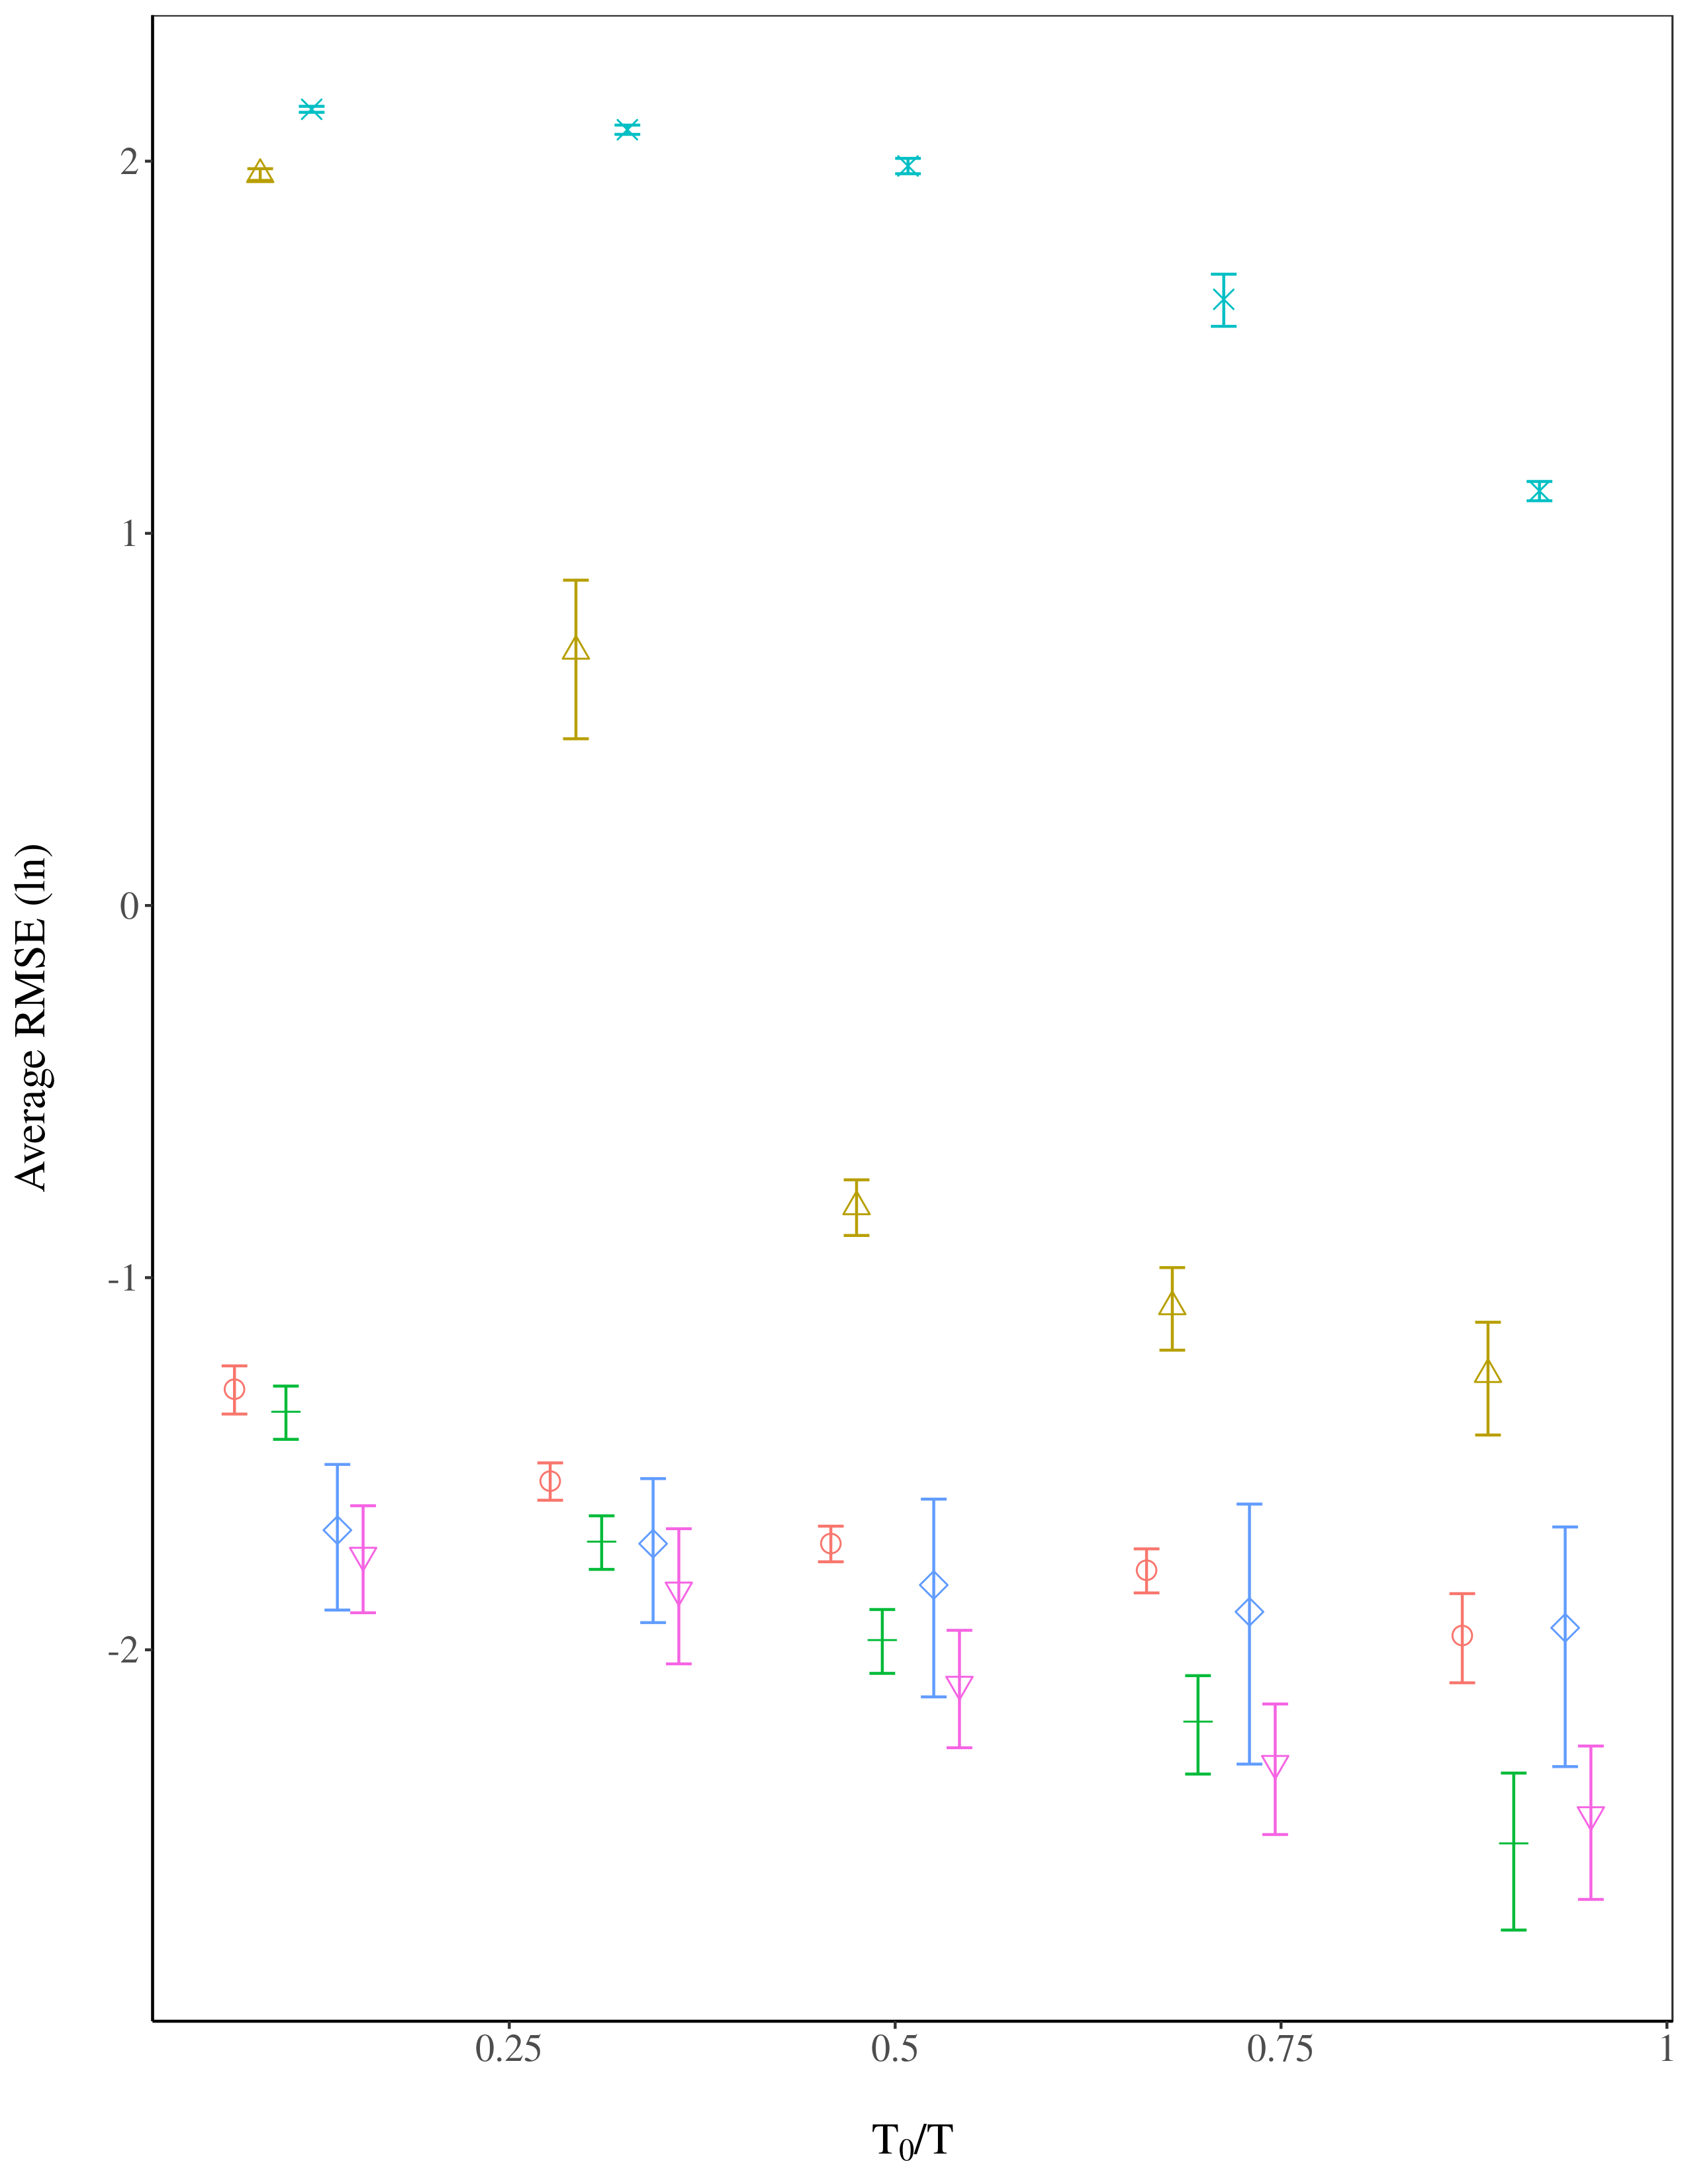
\includegraphics[width=0.9\textwidth]{plots/germany-sim.png}
	\caption{Placebo tests on West German reunification data: 
		{\protect\tikz \protect\draw[color={rgb:red,4;green,0;yellow,1}] (0,0) -- plot[mark=o, mark options={scale=2}] (0.25,0) -- (0.5,0);}, DID;
		{\protect\tikz \protect\draw[color={rgb:red,244;green,226;blue,66}] (0,0) -- plot[mark=triangle*, mark options={scale=2,fill=white}] (0.25,0) -- (0.5,0);}, ED; 
		{\protect\tikz \protect\draw[color={rgb:red,0;green,5;blue,1}] (0,0) -- plot[mark=+, mark options={scale=2}] (0.25,0) -- (0.5,0);}, MC-NNM;
		{\protect\tikz \protect\draw[color={rgb:red,66;green,200;blue,244}] (0,0) -- plot[mark=x, mark options={scale=2}] (0.25,0) -- (0.5,0);}, RVAE;
		{\protect\tikz \protect\draw[color={rgb:red,66;green,107;blue,244}] (0,0) -- plot[mark=diamond, mark options={scale=2}] (0.25,0) -- (0.5,0);}, SCM;
		{\protect\tikz \protect\draw[color={rgb:red,244;pink,66;blue,223}] (0,0) -- plot[mark=triangle, mark options={scale=2, rotate=180}] (0.25,0) -- (0.5,0);}, VT-EN.\label{germany-sim}}
\end{figure}

\begin{figure*}[htbp]
	\centering
	\begin{subfigure}[t]{0.48\textwidth}
		\centering
		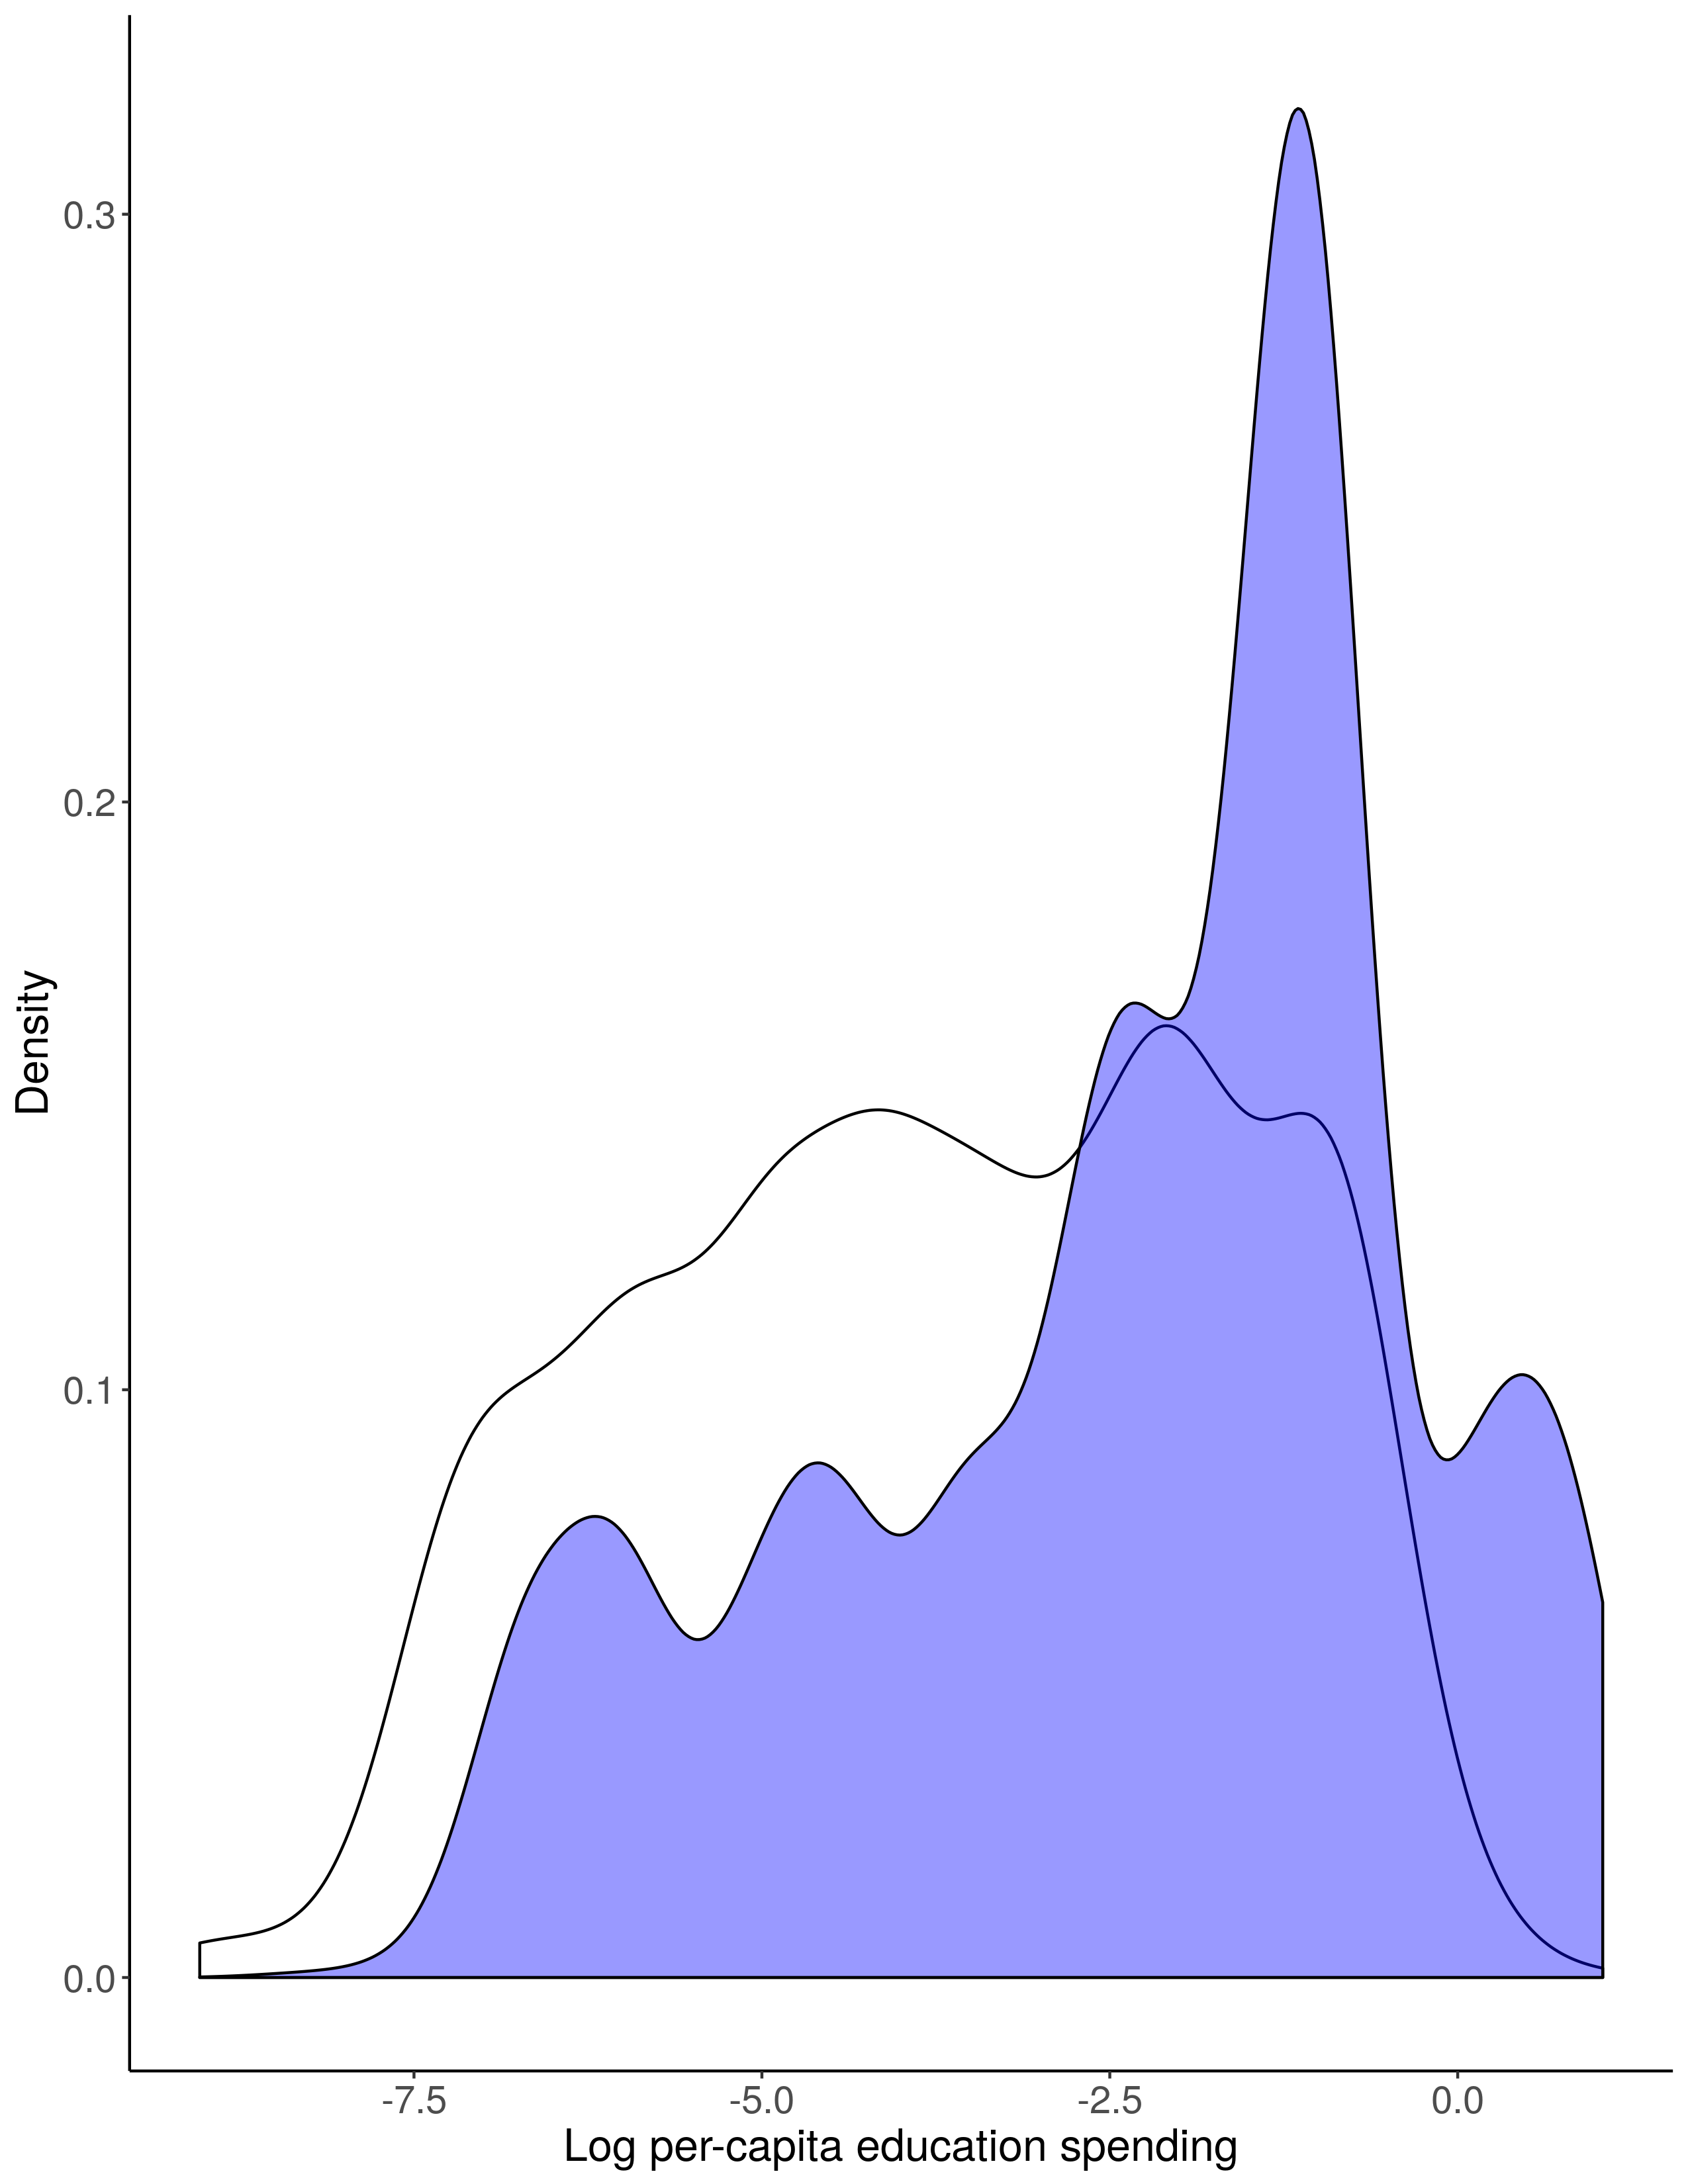
\includegraphics[width=\textwidth]{plots/educ-dens.png}
		\caption{Unweighted} 
	\end{subfigure}
	~ 
	\begin{subfigure}[t]{0.48\textwidth}
		\centering
		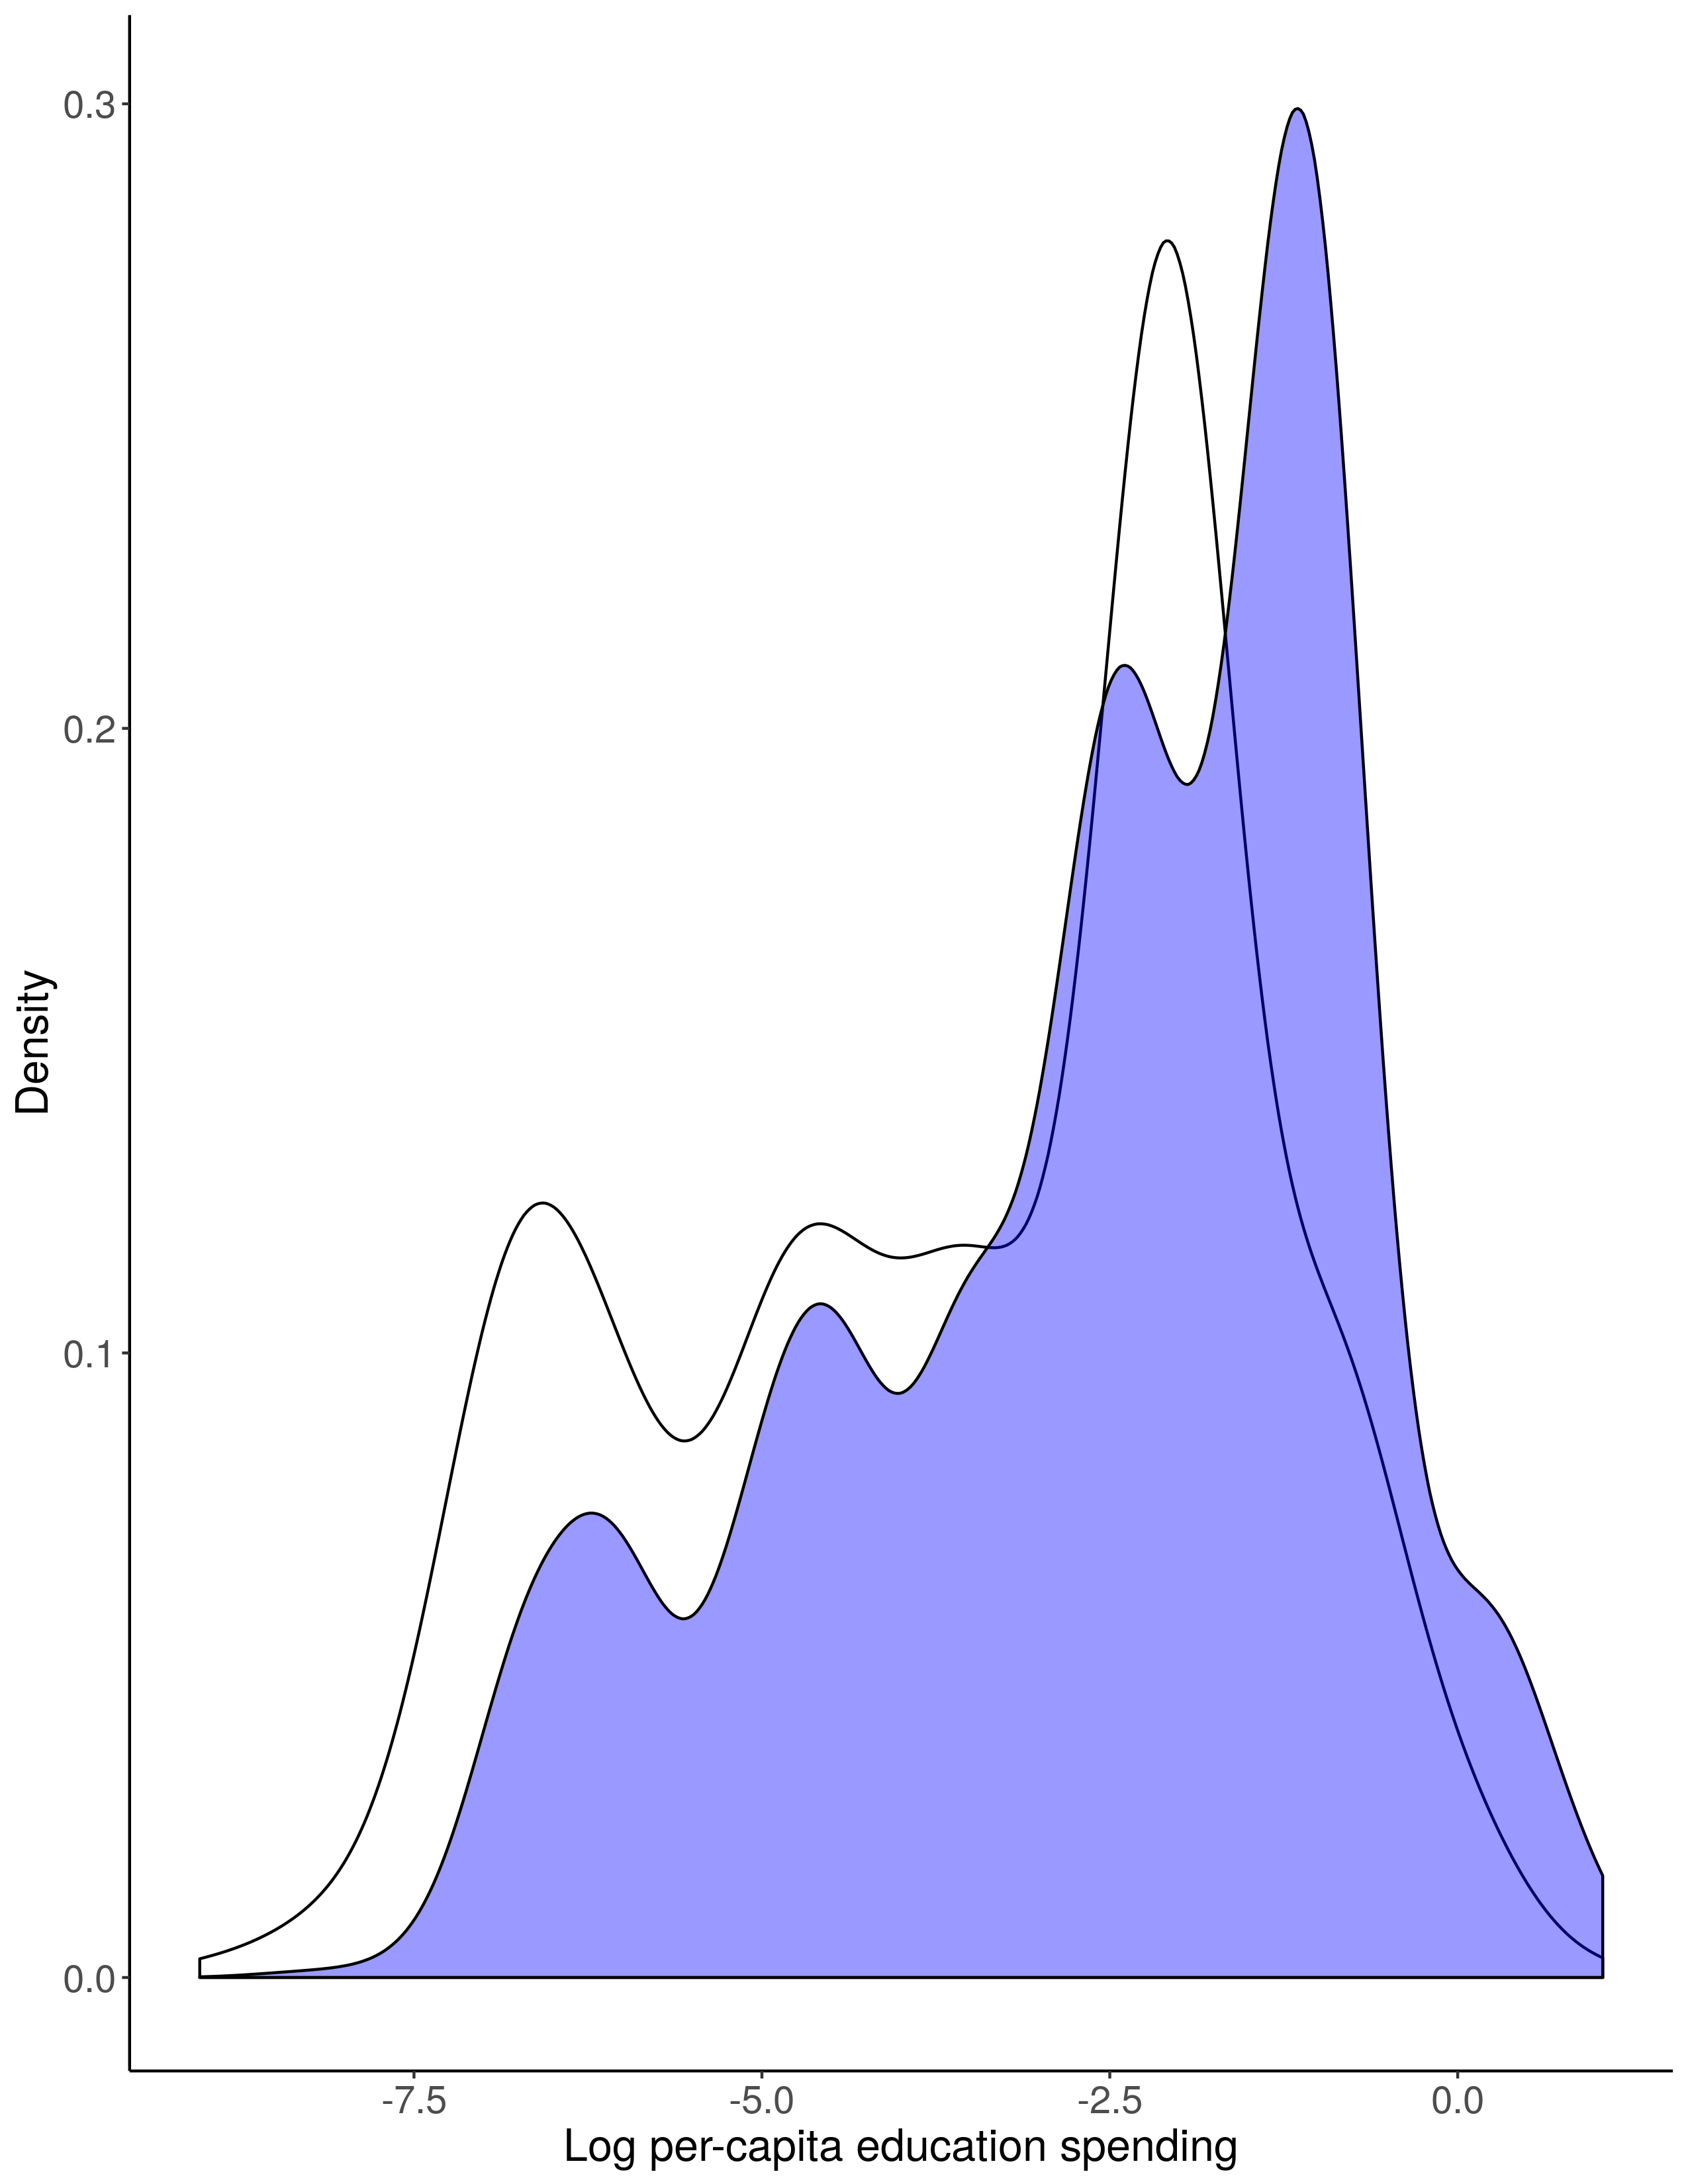
\includegraphics[width=\textwidth]{plots/educ-dens-w.png}
		\caption{Weighted by propensity score}
	\end{subfigure}
	\caption{Pre-period densities of log per-capita state government education spending by treatment status:{\protect\tikz \protect\draw[color=black] (0,0) -- plot[mark=square, mark options={scale=2, fill=white}] (0.25,0) -- (0.5,0);}, Control;
		{\protect\tikz \protect\draw[color={rgb:red,104;green,122;blue,255}] (0,0) -- plot[mark=square*, mark options={scale=2,fill={rgb:red,104;green,122;blue,255}}] (0.25,0) -- (0.5,0);}, Treated \label{educ-dense}} 
\end{figure*}

\begin{figure}[htbp]
	\centering
	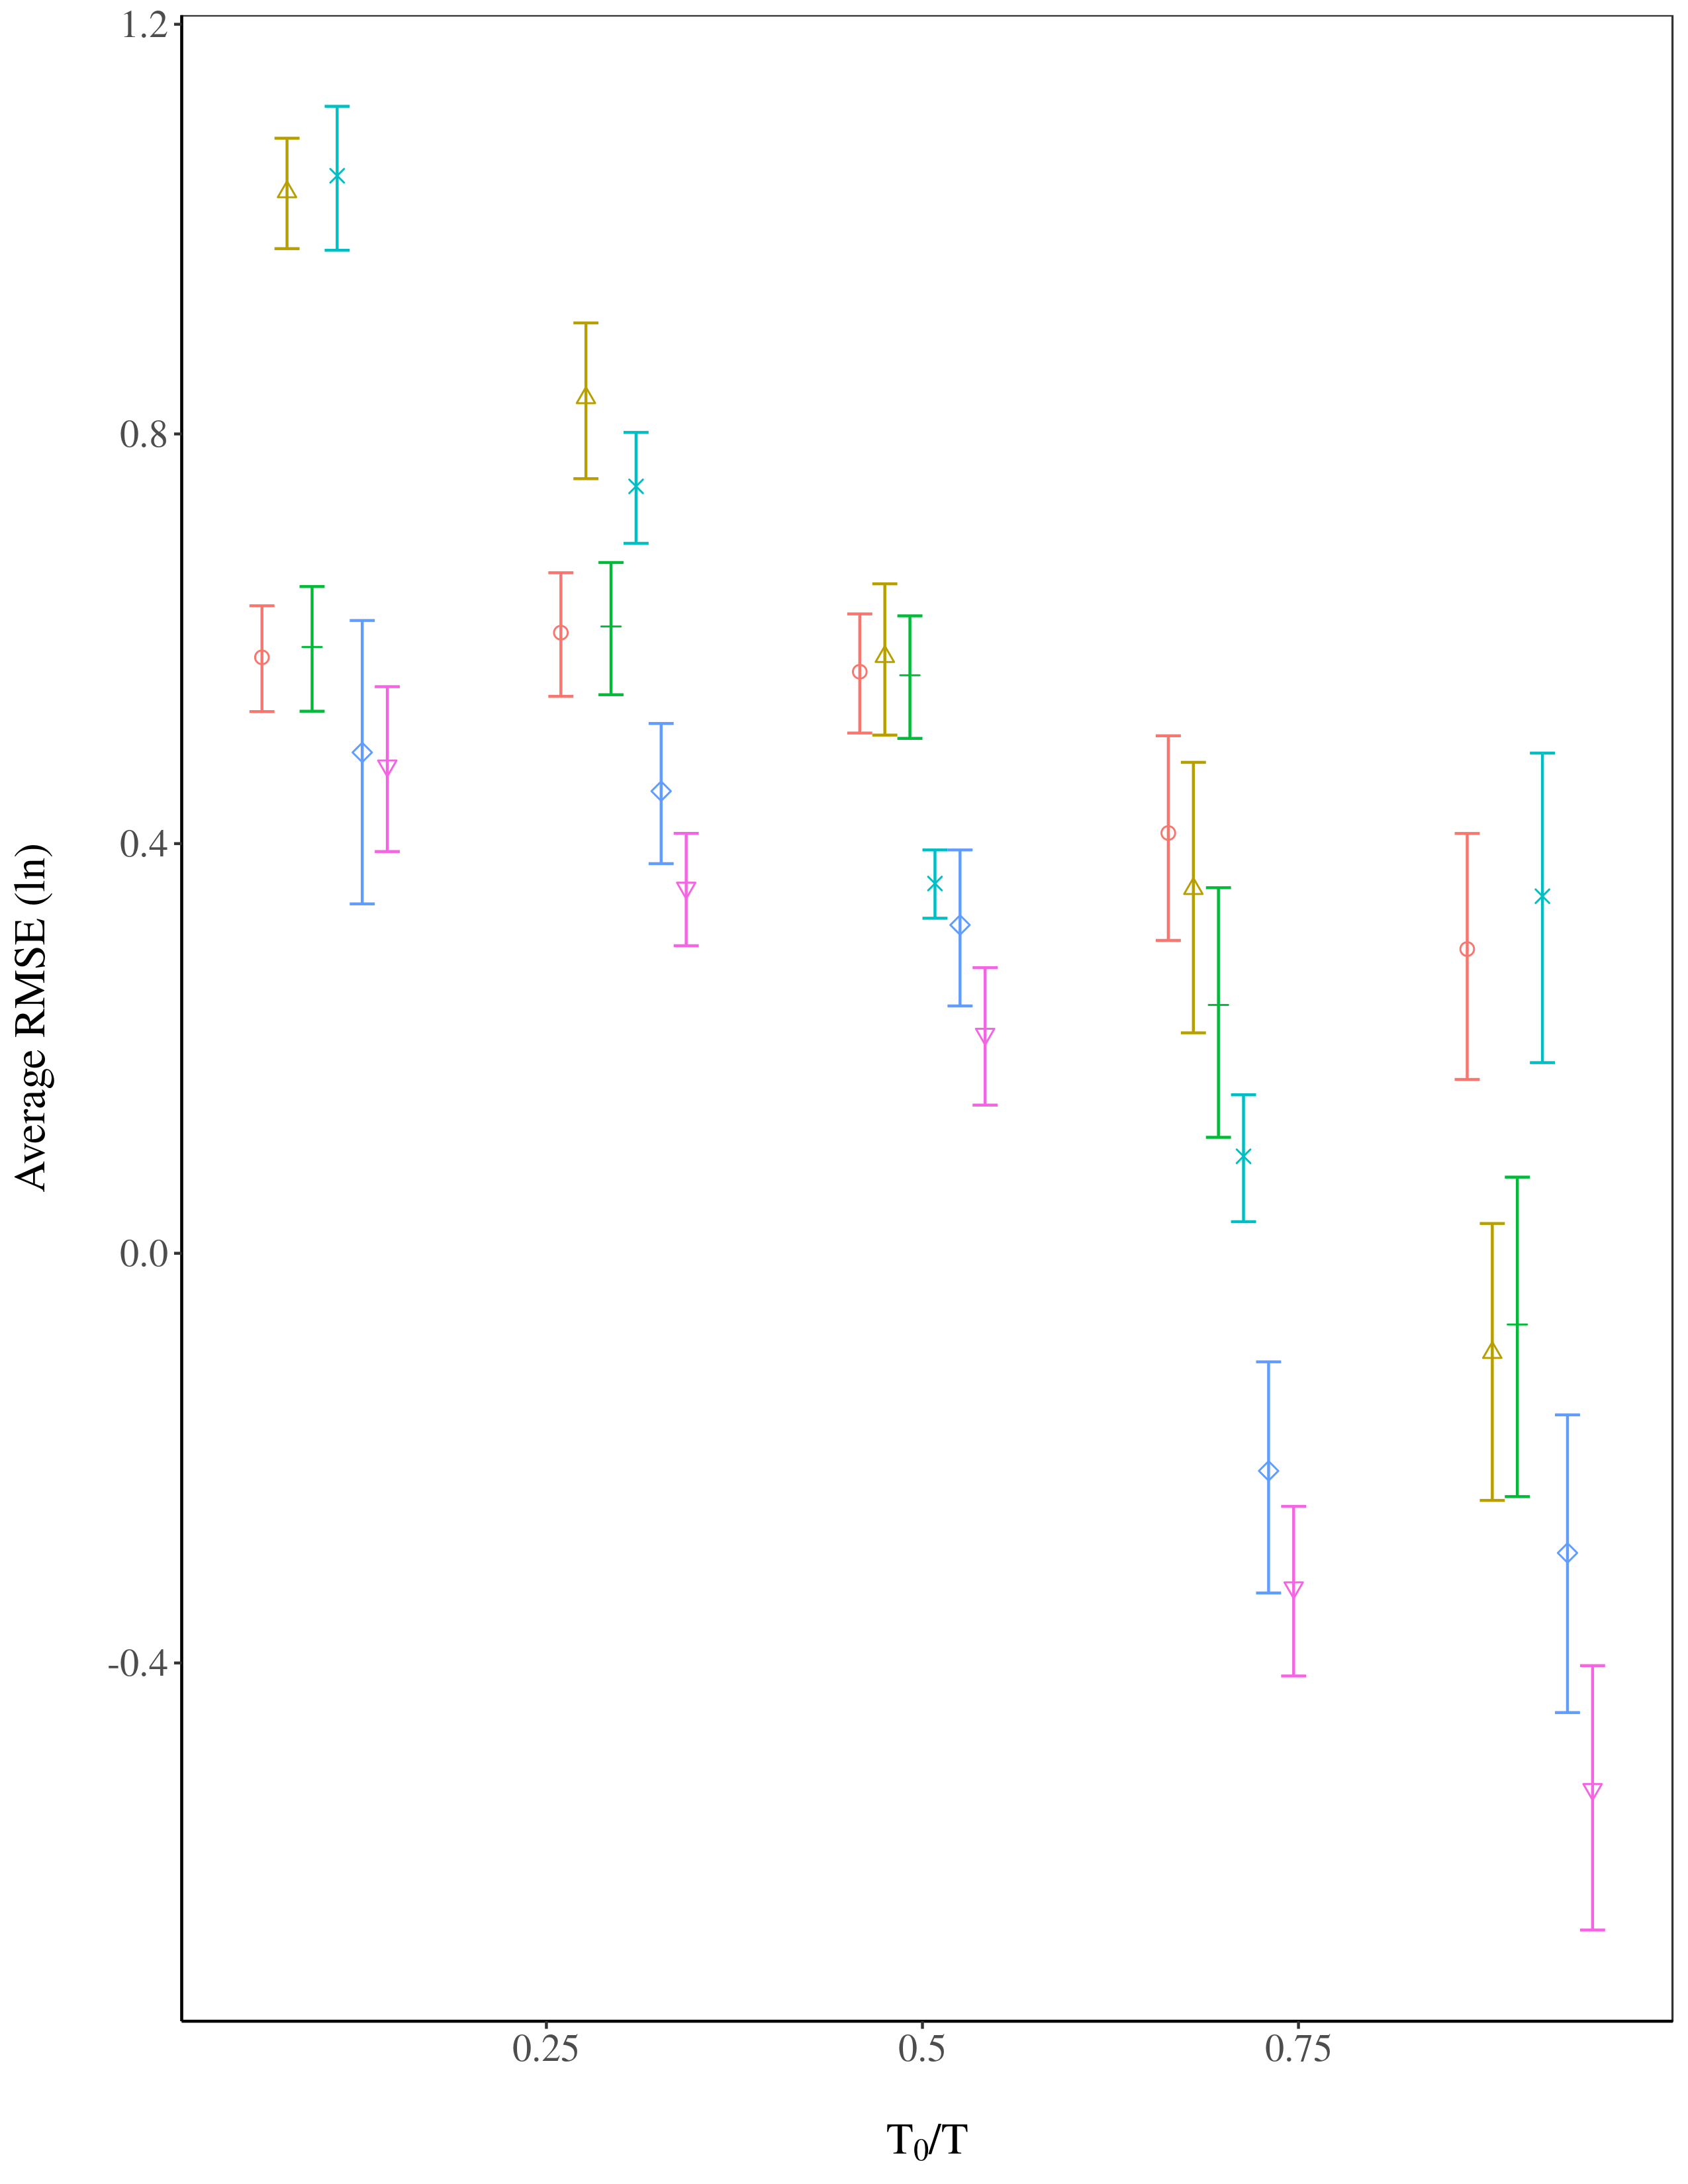
\includegraphics[width=0.9\textwidth]{plots/educ-sim.png}
	\caption{Placebo tests on education spending data: 		{\protect\tikz \protect\draw[color={rgb:red,4;green,0;yellow,1}] (0,0) -- plot[mark=o, mark options={scale=2}] (0.25,0) -- (0.5,0);}, DID;
		{\protect\tikz \protect\draw[color={rgb:red,244;green,226;blue,66}] (0,0) -- plot[mark=triangle*, mark options={scale=2,fill=white}] (0.25,0) -- (0.5,0);}, ED; 
		{\protect\tikz \protect\draw[color={rgb:red,0;green,5;blue,1}] (0,0) -- plot[mark=+, mark options={scale=2}] (0.25,0) -- (0.5,0);}, MC-NNM;
		{\protect\tikz \protect\draw[color={rgb:red,66;green,200;blue,244}] (0,0) -- plot[mark=x, mark options={scale=2}] (0.25,0) -- (0.5,0);}, RVAE;
		{\protect\tikz \protect\draw[color={rgb:red,66;green,107;blue,244}] (0,0) -- plot[mark=diamond, mark options={scale=2}] (0.25,0) -- (0.5,0);}, SCM;
		{\protect\tikz \protect\draw[color={rgb:red,244;pink,66;blue,223}] (0,0) -- plot[mark=triangle, mark options={scale=2, rotate=180}] (0.25,0) -- (0.5,0);}, VT-EN.
		\label{educ-sim}}
\end{figure}

%\begin{figure}[htbp]
%		\centering
%		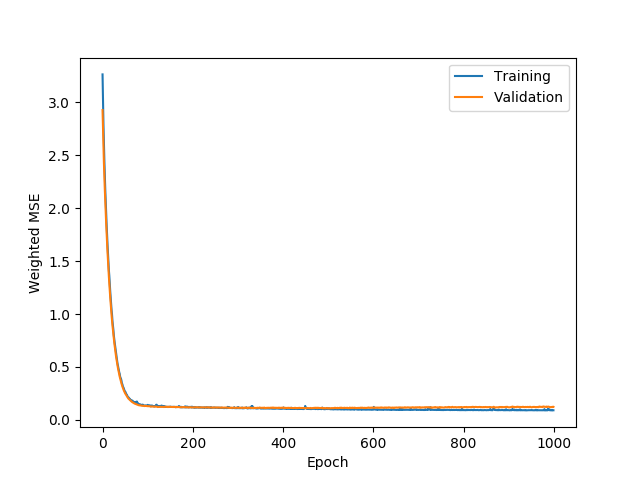
\includegraphics[width=0.9\textwidth]{plots/educ-ed-loss.png}
%%	~ 
%%	\begin{subfigure}[t]{0.8\textwidth}
%%		\centering
%%		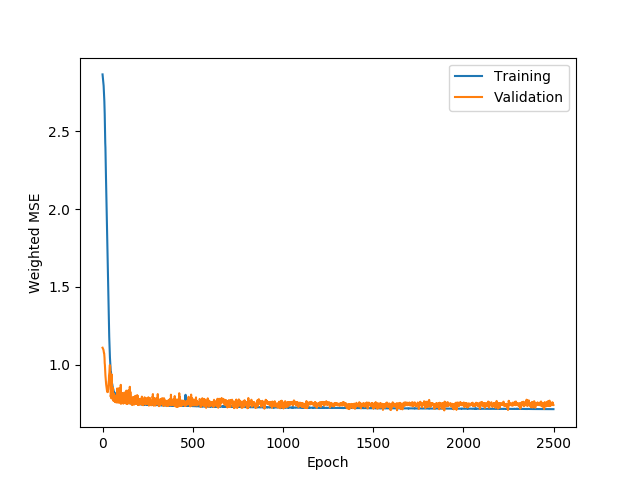
\includegraphics[width=\textwidth]{plots/educ-rvae-loss.png}
%%		\caption{RVAE}
%%	\end{subfigure}
%	\caption{Encoder-decoder networks training and validation loss on education spending data. \label{educ-loss}} 
%\end{figure}

%\begin{figure}[htbp]
%	\centering
%		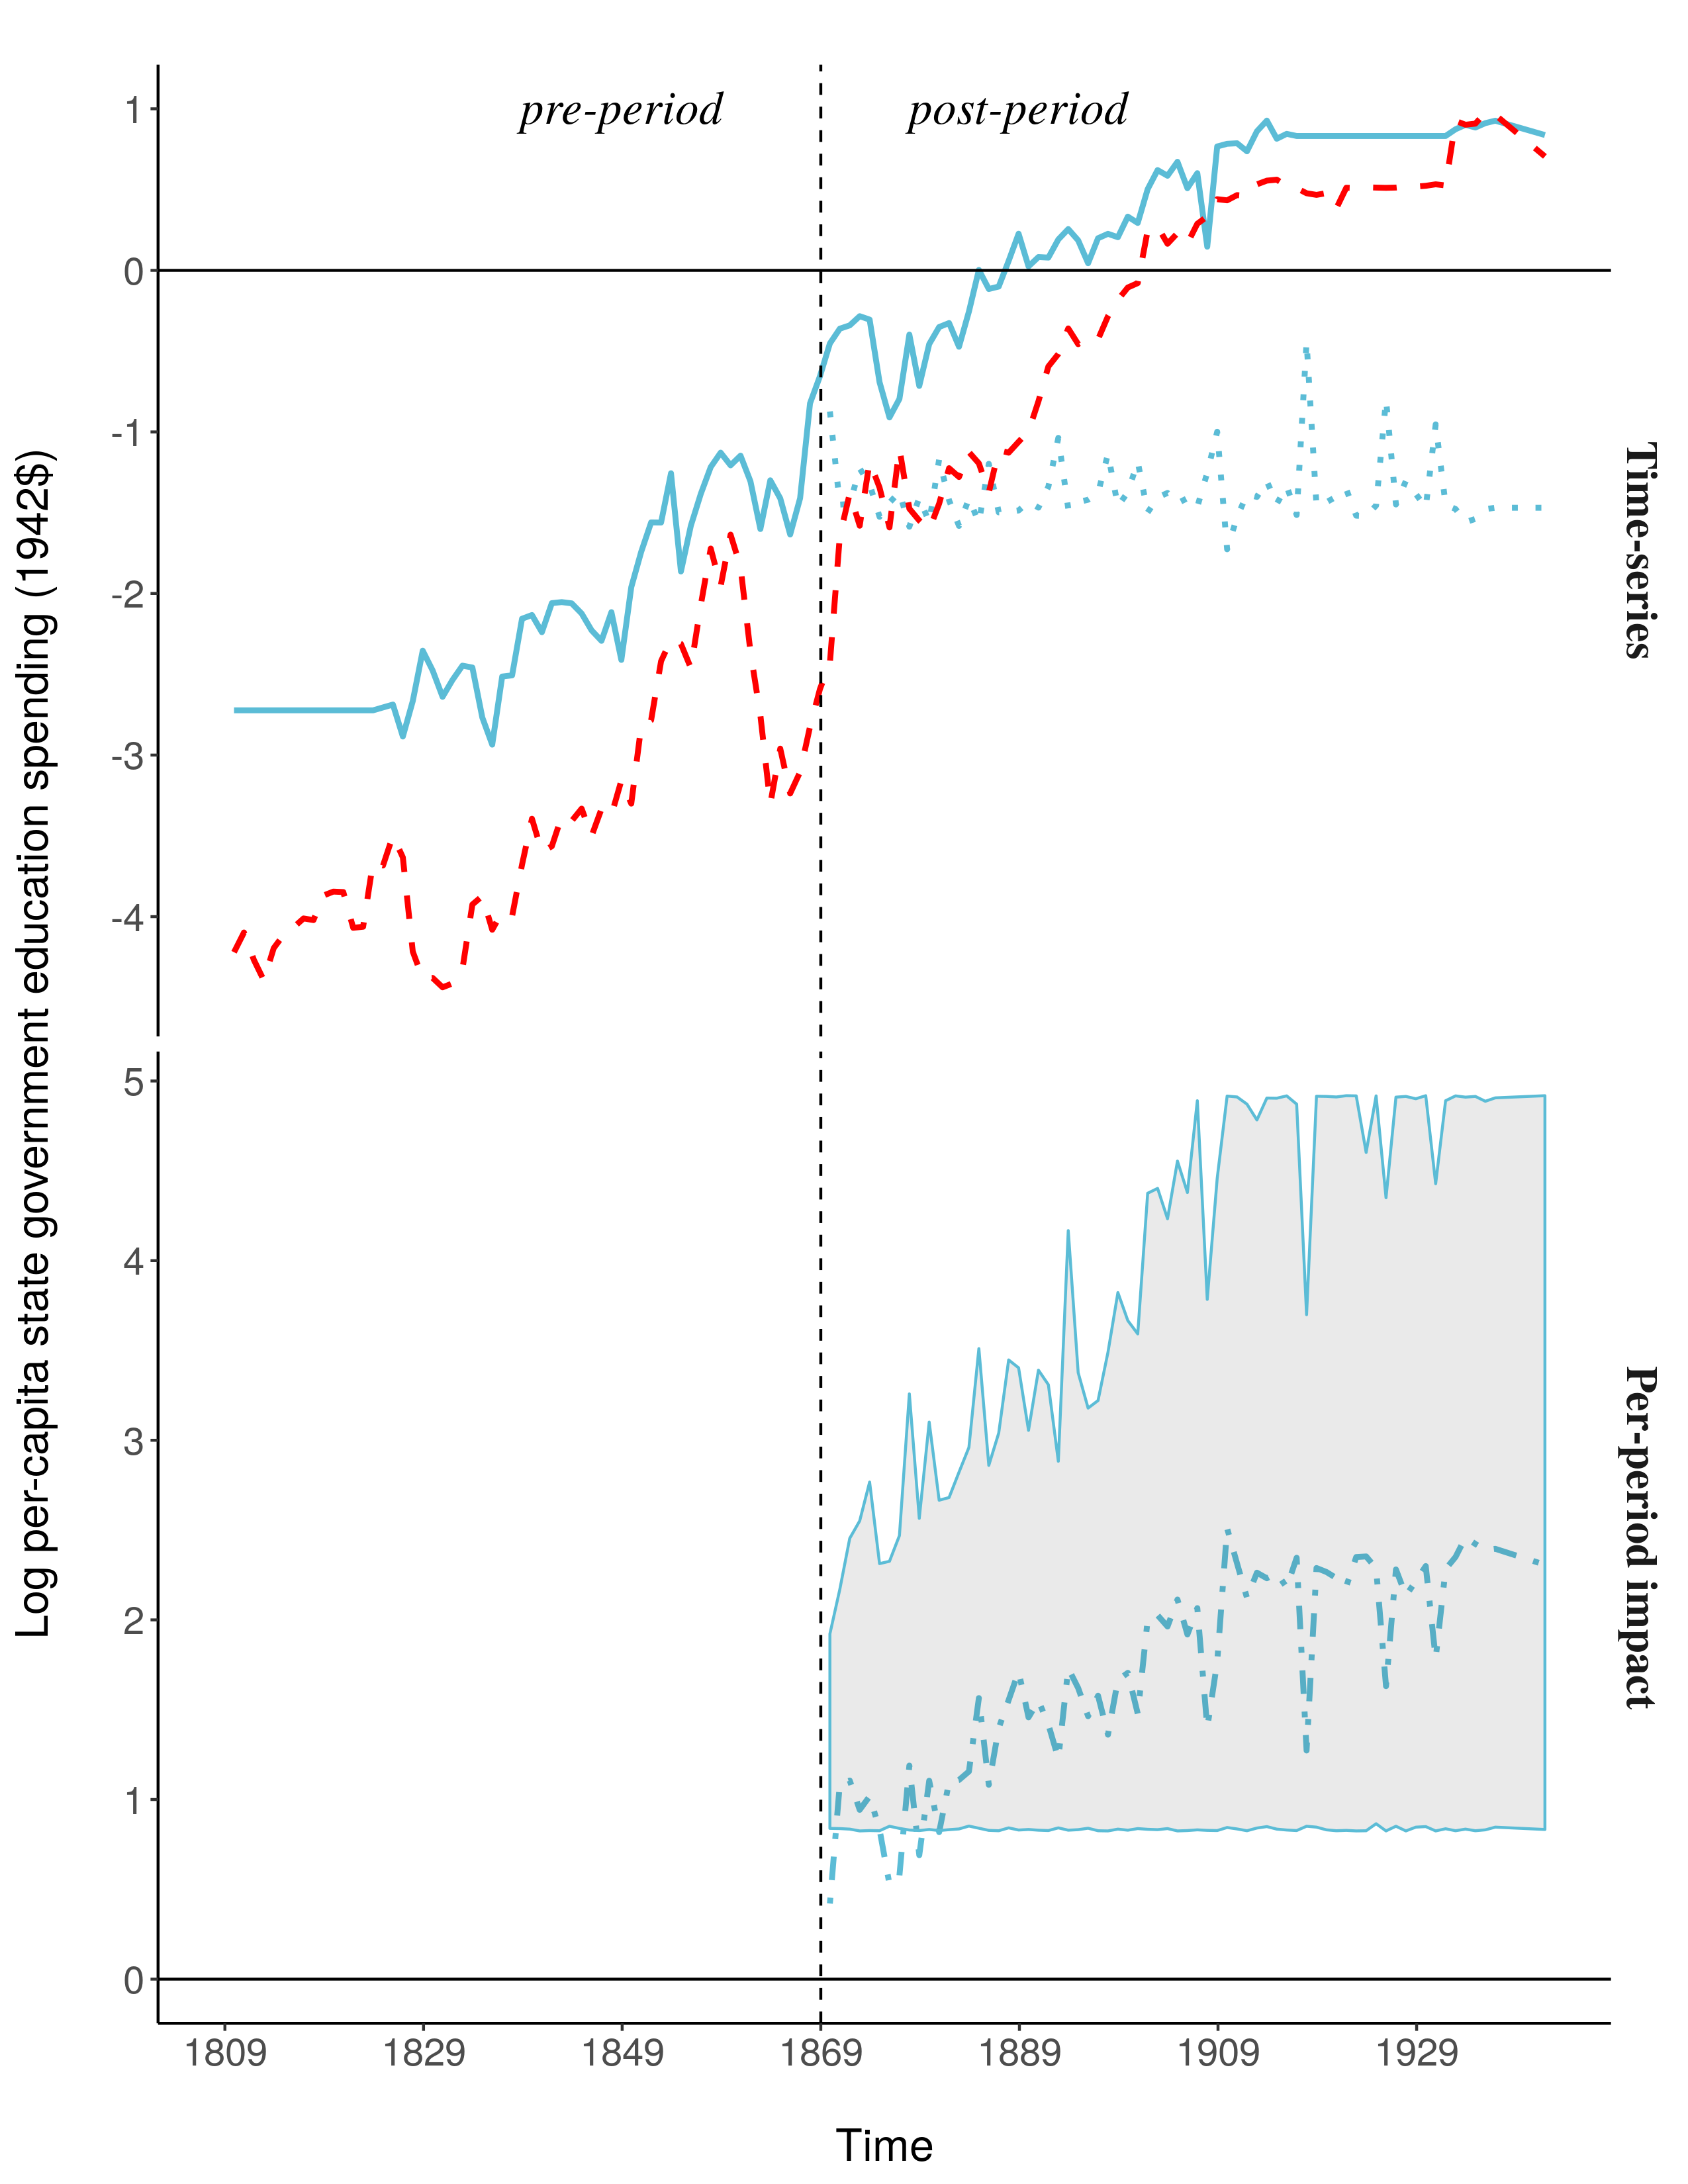
\includegraphics[width=\textwidth]{plots/educ-rvae.png}
%	\caption{RVAE estimates of the homestead act on state government education spending, 1809 to 1982.\label{rvae-ed}} 
%\end{figure}

%\begin{figure}[htbp]
%	\begin{center}
%		\includegraphics[width=0.9\textwidth]{/media/jason/Dropbox/github/land-reform/paper/plots/homestead-heatmap.png}
%	\end{center}
%	\caption{Per-capita homestead entries in state $i$ and year $t$, 1869-1922. \label{fig:homestead-heatmap}}
%\end{figure}

\bibliographystyle{rss}
\begin{singlespace}
\bibliography{rnns-causal-sm}
\end{singlespace}

\itemize
\end{document}
